%% LyX 2.4.4 created this file.  For more info, see https://www.lyx.org/.
%% Do not edit unless you really know what you are doing.
\documentclass[12pt,onecolumn,fleqn,english,compsoc]{IEEEtran}
\usepackage{libertineRoman}
\renewcommand{\sfdefault}{lmss}
\renewcommand{\ttdefault}{lmtt}
\usepackage[T1]{fontenc}
\usepackage{textcomp}
\usepackage[latin9]{inputenc}
\usepackage{parskip}
\usepackage{color}
\usepackage{babel}
\usepackage{booktabs}
\usepackage{amsmath}
\usepackage{amssymb}
\usepackage{graphicx}
\usepackage[bookmarks=true,bookmarksnumbered=true,bookmarksopen=true,bookmarksopenlevel=2,
 breaklinks=false,pdfborder={0 0 0},pdfborderstyle={},backref=false,colorlinks=true]
 {hyperref}
\hypersetup{pdftitle={A simple iterative grid- and density-based Clustering Algorithm},
 pdfauthor={Uwe St�hr},
 pdfsubject={data clustering},
 pdfkeywords={clustering},
 pdfpagelayout=OneColumn,pdfstartview=XYZ,linkcolor=black, citecolor=black}

\makeatletter

%%%%%%%%%%%%%%%%%%%%%%%%%%%%%% LyX specific LaTeX commands.
\newcommand{\noun}[1]{\textsc{#1}}
%% Because html converters don't know tabularnewline
\providecommand{\tabularnewline}{\\}

%%%%%%%%%%%%%%%%%%%%%%%%%%%%%% Textclass specific LaTeX commands.
\newenvironment{lyxlist}[1]
	{\begin{list}{}
		{\settowidth{\labelwidth}{#1}
		 \setlength{\leftmargin}{\labelwidth}
		 \addtolength{\leftmargin}{\labelsep}
		 \renewcommand{\makelabel}[1]{##1\hfil}}}
	{\end{list}}

%%%%%%%%%%%%%%%%%%%%%%%%%%%%%% User specified LaTeX commands.
% enable hyperlinks to subcaptions
\usepackage[figure]{hypcap}
% set caption labels bold and use indentation
\usepackage[labelfont=bf,format=hang]{caption}

% redefine the automatic names for references to labels
\AtBeginDocument{\renewcommand{\ref}[1]{\mbox{\autoref{#1}}}}
\newlength{\abc}
\settowidth{\abc}{\space}
\AtBeginDocument{%
 \renewcommand{\equationautorefname}{\hspace{-\abc}}
 \renewcommand{\itemautorefname}{\hspace{-\abc}}
 \renewcommand{\sectionautorefname}{Sec.\negthinspace}
 \renewcommand{\subsectionautorefname}{Sec.\negthinspace}
 \renewcommand{\subsubsectionautorefname}{Sec.\negthinspace}
 \renewcommand{\figureautorefname}{Fig.\negthinspace}
 \renewcommand{\tableautorefname}{Tab.\negthinspace}
}

% raises threshold above which floats appear on
% one page alone
\renewcommand{\floatpagefraction}{0.7}

% raises threshold above which floats appear at
% bottom of page
\renewcommand{\bottomfraction}{0.5}

% needed for biblatex
\usepackage{csquotes}

% protect some workds from being hyphenated
\hyphenation{DBSCAN}
\hyphenation{DENCLUE}
\hyphenation{CLIQUE}

\ifdefined\showcaptionsetup
 % Caption package is used. Advise subfig not to load it again.
 \PassOptionsToPackage{caption=false}{subfig}
\fi
\usepackage{subfig}
\makeatother

\usepackage[style=numeric,sorting=none]{biblatex}
\addbibresource{biblio/Clustering.bib}
\begin{document}
\title{A simple iterative grid- and density-based Clustering Algorithm}
\author{\IEEEauthorblockN{Uwe St�hr}

\IEEEauthorblockA{Soloof EOOD, Sofia, Bulgaria\\
Email: research\negthinspace{ }@\negthinspace{ }soloof.com\\
Project Page: \href{https://codeberg.org/Soloof/Iteridense}{https://codeberg.org/Soloof/Iteridense}}\vspace{-3\baselineskip}
}
\maketitle
\begin{abstract}
We introduce \noun{Iteridense}, an iterative clustering algorithm
combining grid-based and density-based methods. It provides two possibilities
to perform the clustering and for both it provides a clear path on
how to change the algorithm's input parameters to achieve suitable
results. We show that \noun{Iteridense} is applicable for datasets
with any dimensionality. \noun{Iteridense} provides shorter computation
times than pure density-based algorithms and that it performs clustering
at least as good as the DBSCAN algorithm. We provide a reference implementation
of \noun{Iteridense} as well as a stand-alone program with a graphical
user interface.
\end{abstract}


\section{Introduction}

Density-based clustering algorithms have been proven useful for many
practical applications. There exists a wide variety of algorithms,
some optimized for particular use cases~\cite{Kriegel2011}. However,
these algorithms have a major drawback -- one needs to evaluate neighboring
points for every data point in the dataset to determine if it is part
of a cluster. This is the case for most density-based clustering algorithms
like PreDeCon~\cite{Boehm2004} or HDBSCAN~\cite{Campello2013}.
Other algorithms that combine grid-based with density-based methods
like DENCLUE~\cite{Hinneburg1998} or CLIQUE\,\cite{Agrawal1998}
don't have this drawback but make assumptions about the shape of the
probability distribution of the data (what is the probability to find
a data point inside the range of available data).

Another issue of many clustering algorithms is that as user there
is no clear path on how to change the algorithm's input parameters
to achieve a suitable clustering result. Taking for example the algorithm
DBSCAN~\cite{Ester1996}, it requires to specify the parameter $\epsilon$,
the maximum distance to another core point of a cluster. For many
use cases there is no clear path on how to change $\epsilon$ to get
a suitable result as we will also discuss in this paper.

The algorithm presented in this paper uses both, density-based and
grid-based methods. Its main idea is to work with different probability-density
functions of the dataset and analyzing them in a grid. This approach
makes it possible that even for small datasets in 2~dimensions the
computation can be 10~times faster than a pure density-based algorithm
like DBSCAN. Our algorithm follows an iterative approach to calculate
the probability-density function and makes no assumptions about the
shape of that function. Therefore it provides a clear path on how
to set a start value of the algorithm's main parameter and how to
change it to achieve a certain result.

The algorithm clusters so that no point in a dataset can belong to
more than one cluster. And not all points in the dataset must be assigned
to clusters.

\pagebreak{}

\section{Derivation of the Algorithm\label{sec:Derivation-of-the}}

The basic idea of the algorithm is how mountain peak areas are separated
from each other in a geographical relief. Take for example the relief
shown at the left in \ref{fig:Relief-of-a}. To identify areas around
a peak one cuts the relief at a desired height. The cut-off areas
are then the mountain peak areas. For example in \ref{fig:Relief-of-a}\,(a)
the relief was cut at about 2/3 of the maximal height leading to more
than a dozen peak areas. In \ref{fig:Relief-of-a}\,(b) the relief
was cut at about half the maximal size leading to larger areas. By
decreasing the cutting height, the number of areas will become fewer
unless at a zero height the whole relief area is part of a single
mountain area.

\begin{figure}
\begin{centering}
\subfloat[Cut at 2/3 of its maximal height.]{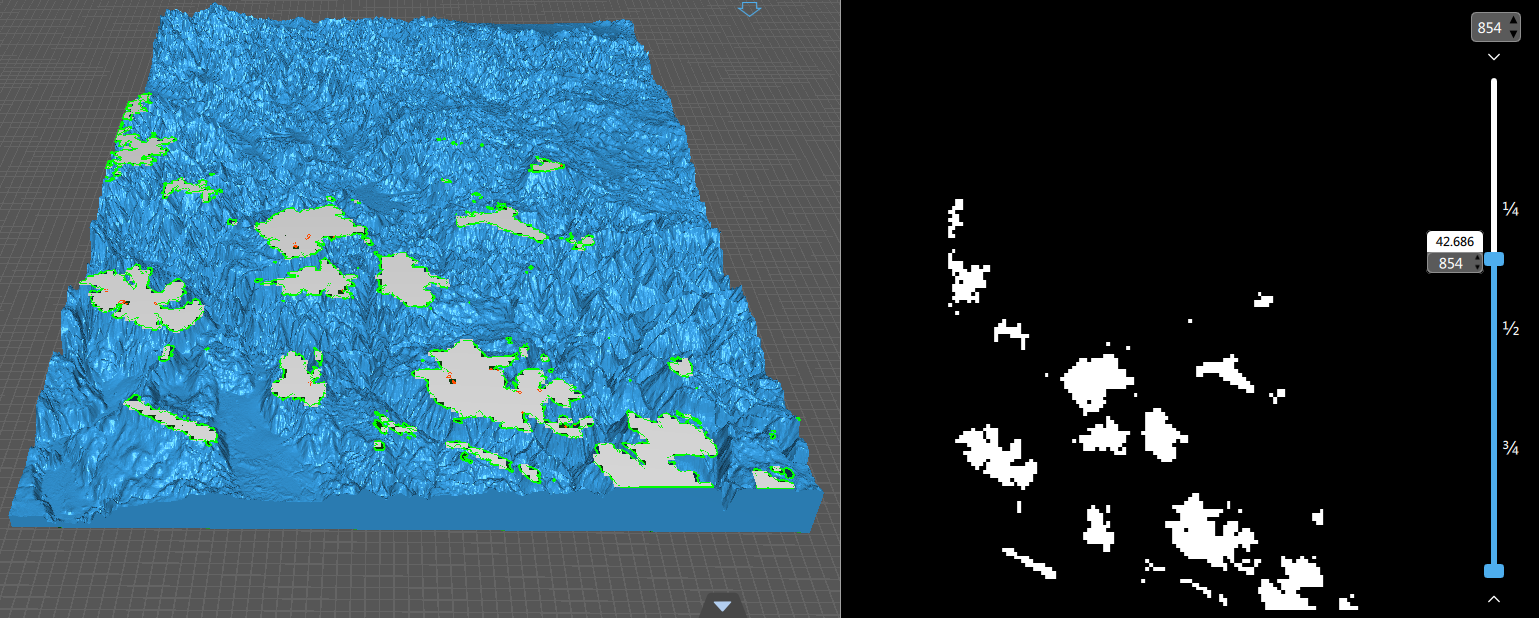
\includegraphics[width=0.75\columnwidth]{clipart/Height-map-layer-854}

}
\par\end{centering}
\begin{centering}
\subfloat[Cut at half of its maximal height.]{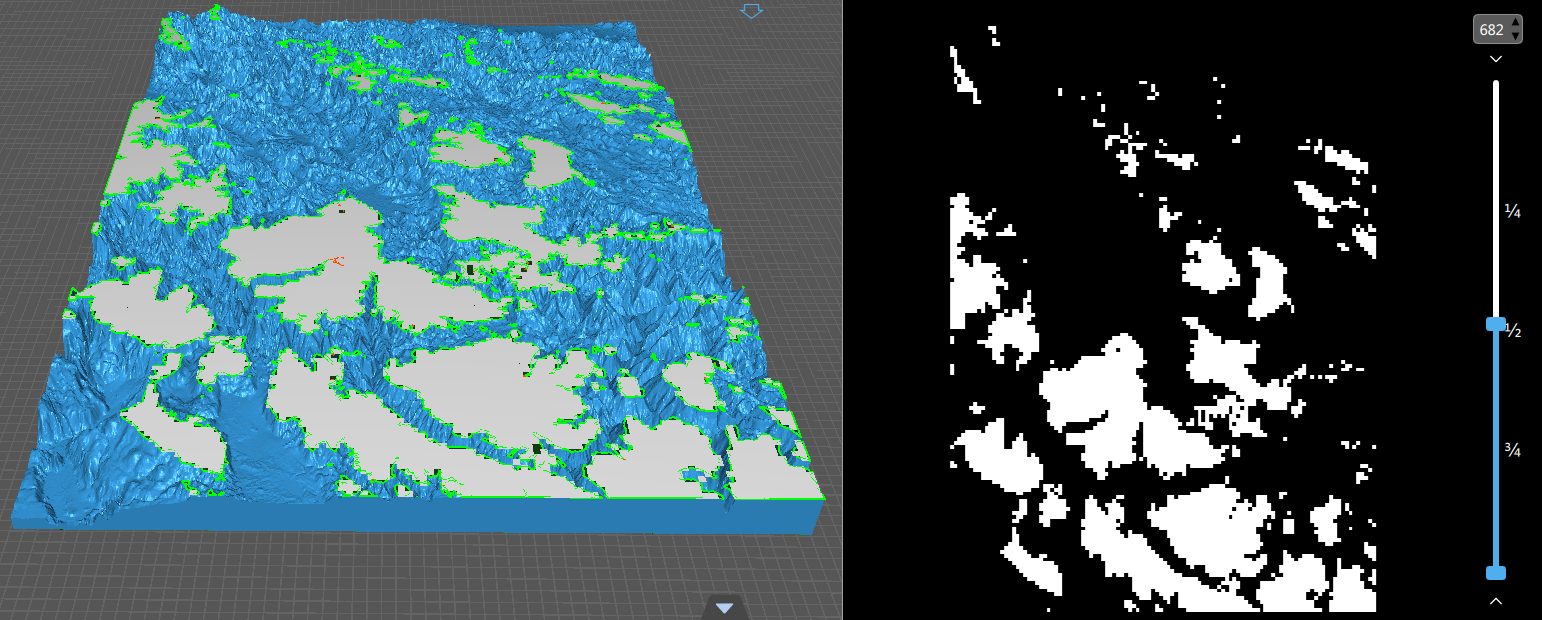
\includegraphics[width=0.75\columnwidth]{clipart/Height-map-layer-682}

}
\par\end{centering}
\caption{\label{fig:Relief-of-a}Relief of a random geographic area cut at
different heights.}
\end{figure}

Translating the relief height to the density of data points $\rho$,
the cut is made at a certain $\rho$ through the probability-density
function of the dataset. See also the section \emph{Background and
Motivation} of \cite{Kriegel2011} for a similar visualization than
in \ref{fig:Relief-of-a}.

Detecting clusters by making a cut through the probability-distribution
is state-of-the-art \cite{Kriegel2011}. The novelty is how to generate
the distribution and how to cut it. Instead of calculating a single
probability-density function, we calculate different probability-density
functions in an iterative process with increasing resolutions. Resolution
means hereby into how many cells every dimension of the dataset is
divided to calculate the probability-density function. For every resolution
a clustering of the cells is performed and one gets two results: the
amount of clusters and the density of every cluster. Depending on
the results, the algorithm is stopped, or it continues and calculates
another probability-density function at a higher resolution.

We call our algorithm \noun{Iteridense} (ITERative grID- and dENSity-basEd
clustering). Based on our approach the key features of \noun{Iteridense}
are:
\begin{itemize}
\item The clustering works without the need to test neighbors of every data
point, making the clustering more computation-efficient. The clusters
are derived by counting the numbers of data points within a certain
data area.
\item One has two choices to stop the algorithm. Either one specifies $\rho$,
the minimal density every found cluster must have to stop the algorithm,
or \textbf{MinClusters}, the number of how many clusters should at
least be detected (in that case the specification of $\rho$ is not
necessary). The possibility to specify \textbf{MinClusters} is a big
advantage compared to pure density-based algorithms that by design
cannot have this feature.
\item For \noun{Iteridense} $\rho$ is defined being normalized so that
the whole dataset has $\rho=1$. Because of the iteration with increasing
resolutions our algorithm provides a clear path on how to set and
change $\rho$: Start with a low $\rho>1$ and increase $\rho$ until
you get a suitable result. The algorithm stops at a resolution that
fulfills the specification of $\rho$. We will demonstrate this feature
with an example in \ref{subsec:Clustering-Performance}.
\end{itemize}

\section{Description of the Iteridense Clustering Algorithm}

\subsection{Basic Algorithm}

There are two possible input parameters to the algorithm, either to
specify how many clusters should at least be detected (\textbf{MinClusters})
or the minimal data point density $\rho$ to form a cluster. $\rho$
is treated as a dimensionless number since the dimension of the data
point space can be anything, depending on the source of the data points.

\ref{fig:Clustering-process}\,(a) shows as example a 2-dimensional
dataset which represents the relative humidity and temperature of
air inside a thermal cabinet after a certain chemical process. It
looks like there might be a cluster of points inside an area in form
of a quarter circle. To find that potential cluster \noun{Iteridense}
works on this dataset the following way:

\begin{figure}
\begin{centering}
\subfloat[Data to be clustered.]{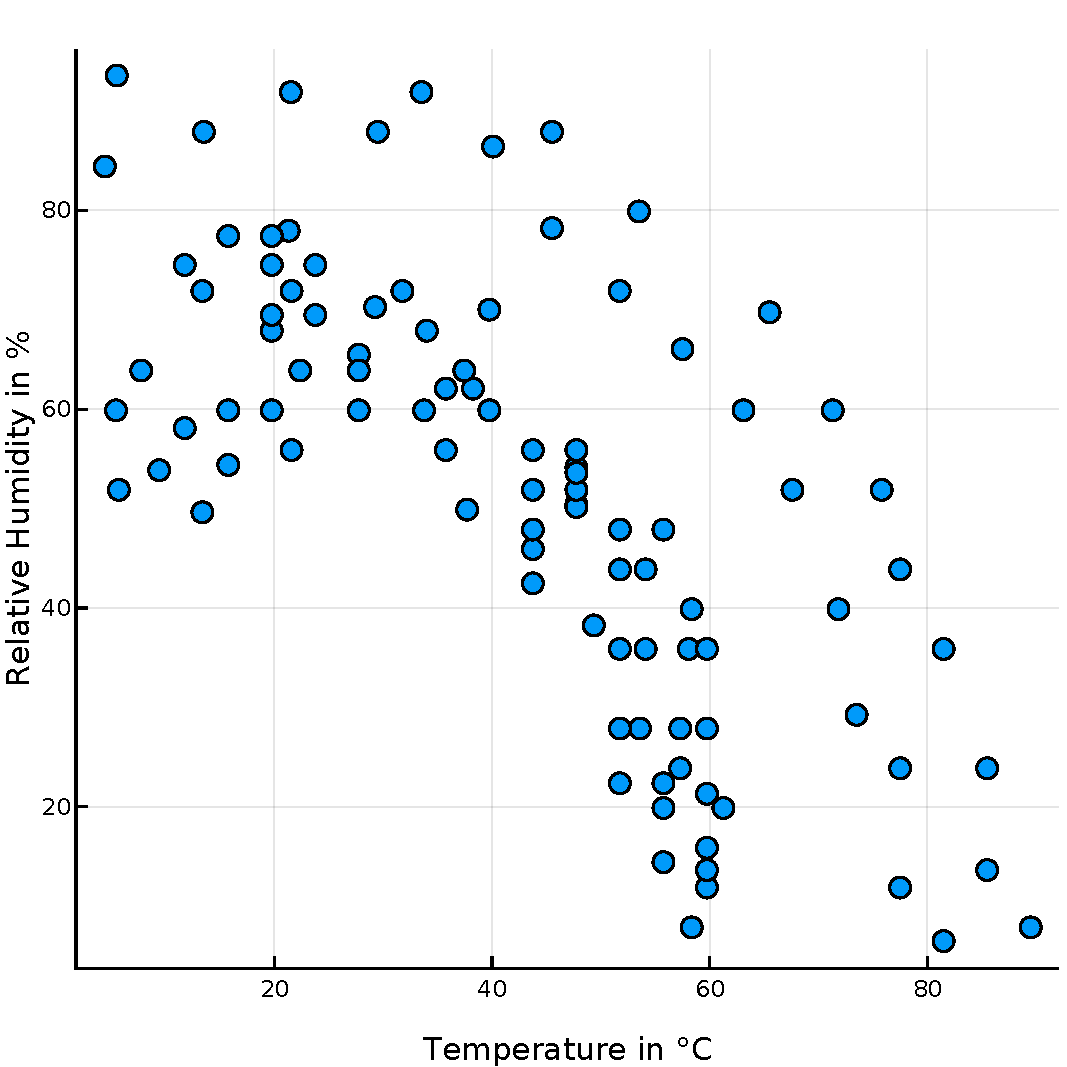
\includegraphics[width=0.33\columnwidth]{clipart/Temperature-initial}

}\subfloat[Count map generated in\protect \\
algorithm step~\ref{enu:AlgoStep3}.]{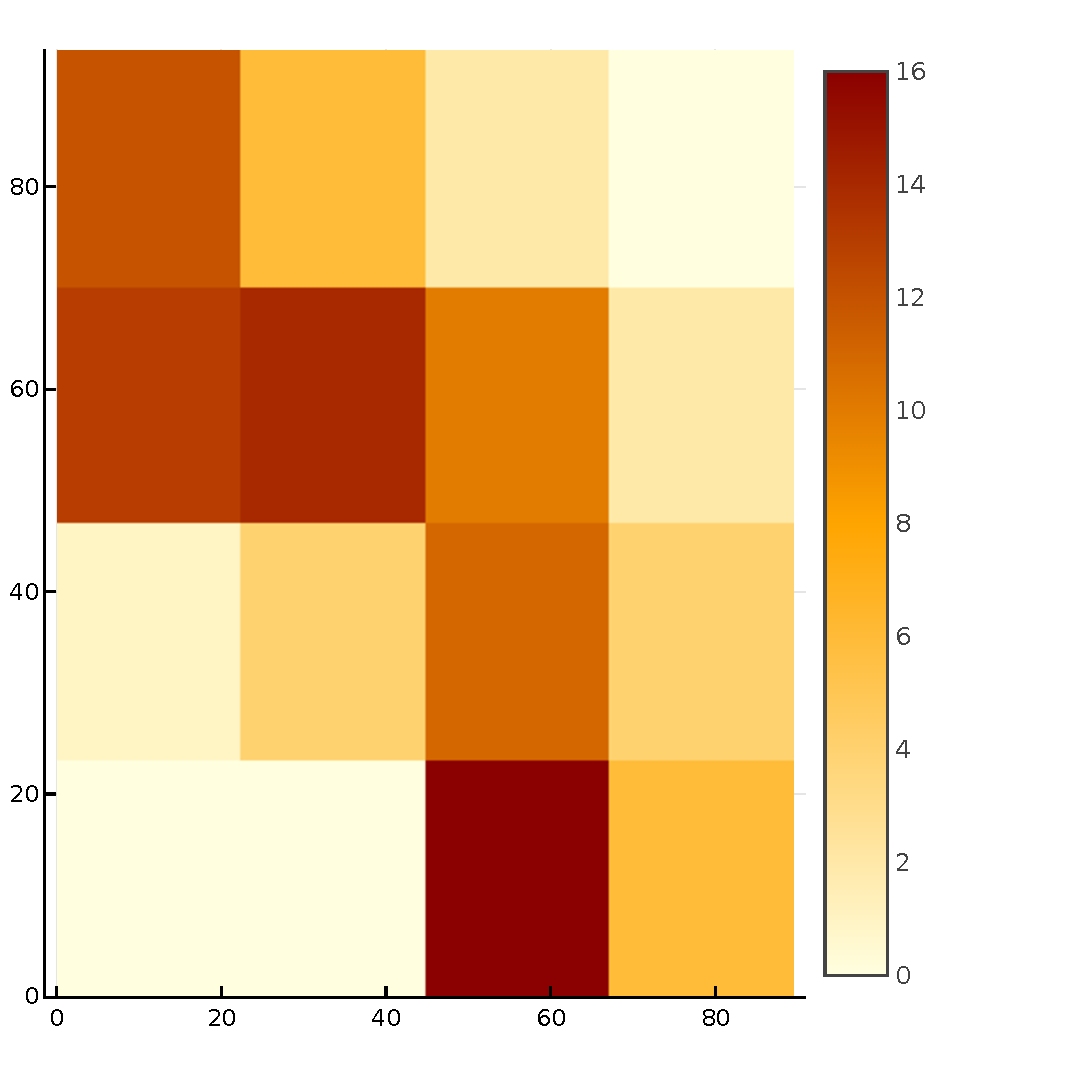
\includegraphics[width=0.33\columnwidth]{clipart/Temperature-4x4-countmap}

}\subfloat[Clustering scheme of the count map.]{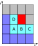
\includegraphics[width=0.29\columnwidth]{clipart/Clustering-Scheme}

}
\par\end{centering}
\caption{\label{fig:Clustering-process}Clustering process of \noun{Iteridense}.
(a) Data to be clustered; (b) Count map generated in algorithm step~\ref{enu:AlgoStep3}
for resolution 4: 16~cells with the info how many data points are
in.; (c) Clustering scheme of the count map. The red cell is the currently
evaluated cell, the blue cells have already be evaluated, cells~A\,--\,D
are neighboring cells determining the clustering for the red cell.}
\end{figure}

\begin{enumerate}
\item \label{enu:AlgoStep1}The space of the dataset is divided into a grid
of 4\,\texttimes \,4~cells. In our example the data range in dimension~1
``temperature'' is 4\,--\,89\,�C and the range in dimension~2
``humidity'' is 6\,--\,93\,\%. These ranges define the space
of the dataset. As we divide into 4\,\texttimes \,4~cells, cell~1
covers the space of temperature range 4\,--\,25.25\,�C and humidity
range 6\,--\,27.75\,\%.\\
A division into 4\,\texttimes \,4~cells is defined as a resolution
of 4. A division into 5\,\texttimes \,5~cells would be a resolution
of 5 and so on.
\item The number of data points in the cells are counted. The result is
a count map as shown in \ref{fig:Clustering-process}\,(b).
\item \label{enu:AlgoStep3}Now the actual clustering is performed. The
evaluating scheme is depicted in \ref{fig:Clustering-process}\,(c).
Every cell is evaluated one after another first in x- then in y-direction.
The most basic definition of a cluster is that a cluster consists
of at least one cell that has at least 2~data points. Therefore,
if a cell has more than 1~data point it could either be a sole cluster
or part of a cluster. To decide this, its neighboring cells are evaluated.
Thereby only those neighbors are evaluated that have already been
evaluated (blue and light-blue in \ref{fig:Clustering-process}\,(c))
because for them it is already known to which cluster they belong
to.

If none of the neighbor cells A\,--\,D are in a cluster, the current
cell will start a new cluster. If any neighbor is in a cluster, the
current cell will become part of that cluster. If neighbor cells are
in different clusters, these clusters are merged and the current cell
becomes part of that merged cluster. For example cell\,A and cell\,C
could be in different clusters and the current cell unites both clusters.
\item The density of every cluster $\rho_{\mathrm{cluster}}$ is calculated
as the number of points in the cluster divided by the number of cells
in the cluster.
\begin{equation}
\rho_{\mathrm{cluster}}=\frac{\text{num points in cluster}}{\text{num cells of cluster}}
\end{equation}
To make $\rho_{\mathrm{cluster}}$ independent of the resolution,
it has to be the normalized.\\
For dimension $>2$:
\begin{equation}
\rho_{\mathrm{cluster}}=\frac{\text{num points in cluster}}{\text{num cells of cluster}}\cdot\frac{\text{total num of points}}{\text{total num of cells}}\cdot\frac{\text{dimension}}{2\thinspace\text{resolution}^{\text{dimension}-2\vphantom{\hat{A}}}}
\end{equation}
For dimension $<3$:
\begin{equation}
\rho_{\mathrm{cluster}}=\frac{\text{num points in cluster}}{\text{num cells of cluster}}\cdot\frac{\text{total num of points}}{\text{total num of cells}}
\end{equation}

The normalization is derived in \ref{subsec:Density-Normalization}.
For less than 3~dimensions $\rho_{\mathrm{cluster}}$ expresses by
what factor the cluster is more dense than the whole dataset.

The final density $\rho_{\mathrm{final}}$ is the minimum of all $\rho_{\mathrm{cluster}}$.
\item \label{enu:AlgoStep5}All clusters are evaluated. Optionally clusters
with $\rho_{\mathrm{cluster}}$ lower than a specified value will
be deleted. If they contain fewer data points than a specified value,
they are deleted as well. See the next section for a description of
these optional settings. The result of this algorithm step is a set
of clusters that are subsequently numbered.
\item The resolution is incremented by one and the steps \ref{enu:AlgoStep1}\,--\,\ref{enu:AlgoStep5}
are repeated until either $\rho_{\mathrm{final}}>\rho$ or until as
many clusters were detected as specified as \textbf{MinClusters}.
To assure that the steps are not repeated forever, the loop is stopped
if the resolution reaches the total number of points in the dataset.
The resolution reached at the end of this step is the final resolution.
\item All data points are assigned according to the found clusters. Points
in cluster ``0'' are hereby not part of a cluster.
\item \label{enu:AlgoStep8}Due to the grid generated in step~\ref{enu:AlgoStep1},
single points might appear in the corner of a cell and are thus not
detected as part of a cluster. Therefore steps \ref{enu:AlgoStep1}\,--\,\ref{enu:AlgoStep5}
are repeated with the final resolution plus 1.
\item Points that were before step~\ref{enu:AlgoStep8} not part of a cluster
but now are, are finally assigned to that cluster. This will only
be done if the number of clusters did not change in step~\ref{enu:AlgoStep8}
and if no data point belongs now to another cluster than before step~\ref{enu:AlgoStep8}.
\end{enumerate}
\ref{fig:Result-Iteridense} shows the result for $\rho=3.0$. In
that case the final resolution is 13 and there is one cluster with
$\rho_{\mathrm{cluster}}=4.3$. Note that this case is just an example
for the algorithm. A suitable clustering result for this dataset would
probably be one with 2~clusters. We will discuss later what ``suitable''
means.

\begin{figure}
\begin{centering}
\hfill{}\subfloat[Resulting data point assignment.]{\begin{centering}
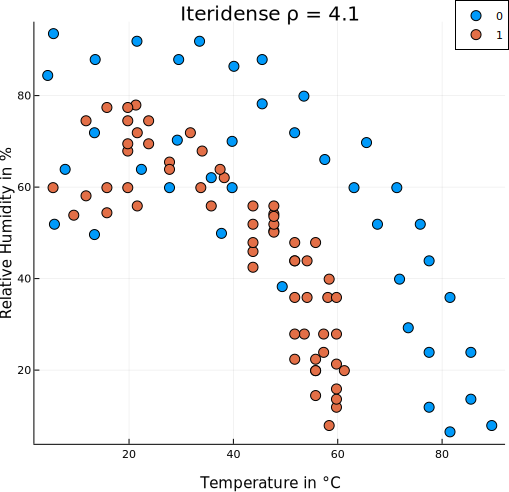
\includegraphics[scale=0.4]{clipart/Temperature-final}
\par\end{centering}
}\hfill{}\subfloat[Final count map (resolution 13).]{\begin{centering}
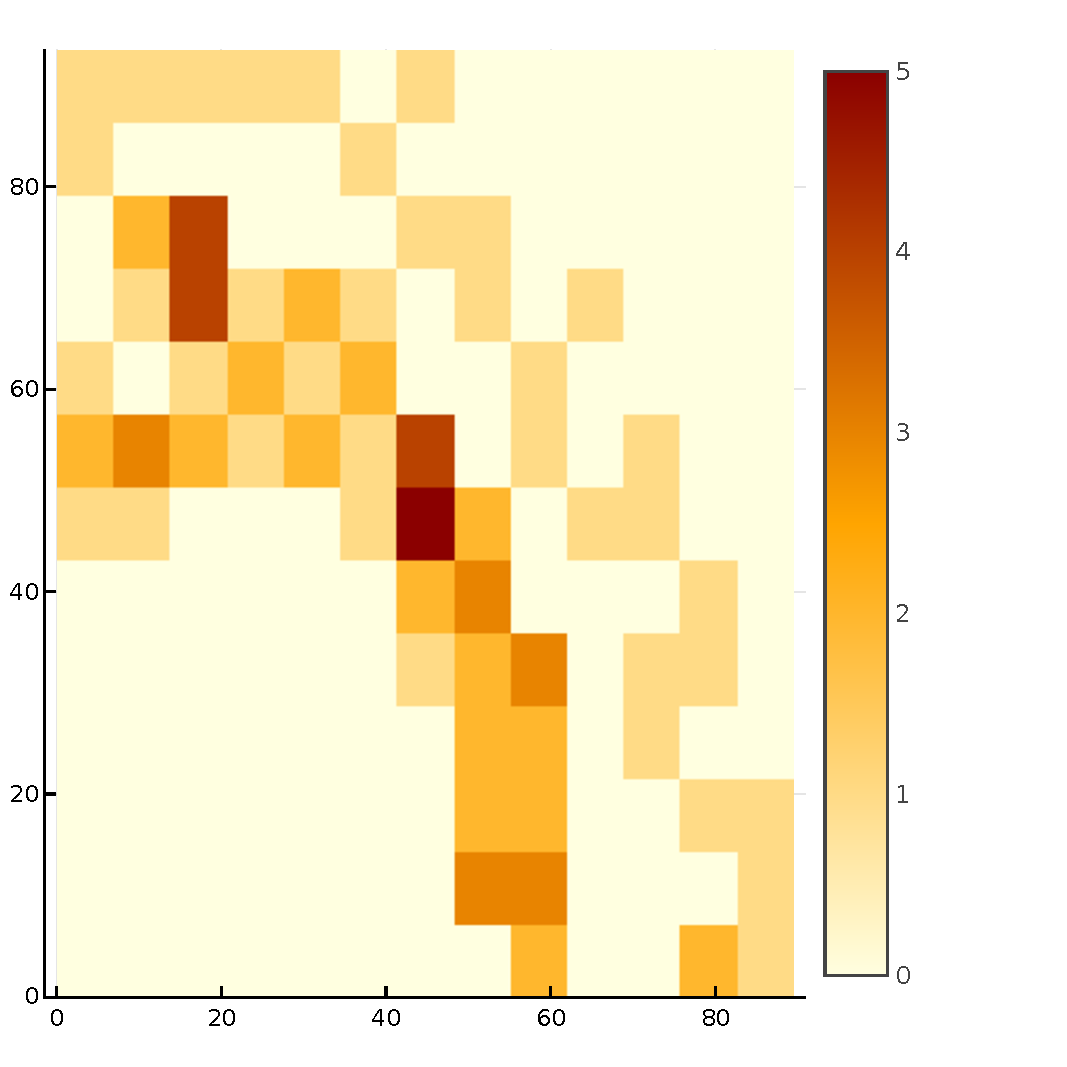
\includegraphics[scale=0.4]{clipart/Temperature-13x13-countmap}
\par\end{centering}
}\hfill{}
\par\end{centering}
\caption{\label{fig:Result-Iteridense}Result of \noun{Iteridense} for the
data shown in \ref{fig:Clustering-process}\,(a) for $\rho=3.0$.}
\end{figure}


\subsection{Optional Settings}

The algorithm can optionally be modified this way:
\begin{enumerate}
\item \label{enu:OptionDiagonal}In step~\ref{enu:AlgoStep3} don't take
cells into account that are diagonally connected to the current cell\\
(\textbf{NoDiagonals}). In \ref{fig:Clustering-process}\,(b) cells~A
and C would then not be evaluated.
\item \label{enu:Specification-of-the}Specification of the start resolution
for step~\ref{enu:AlgoStep1} (\textbf{StartResolution}). The default
and minimum is 2, the maximum is the total number of points in the
dataset.
\item \label{enu:Specification-of-a}Specification of a resolution at which
the loop step~\ref{enu:AlgoStep1}\,--\,\ref{enu:AlgoStep5} is
stopped (\textbf{StopResolution}). It is by default set to $\min(64,N)$,\footnote{Using 64 as default limit is a choice based on practical experience.}
whereas $N$ is the number of data points.
\item \label{enu:OptionClusterSize}Specification of the minimal number
of data points in a cluster (\textbf{MinClusterSize}). Clusters with
less points will be erased. The default is 3, the minimum is 2, the
maximum is the total number of points in the dataset minus 1.
\item \label{enu:OptionClusterDensity}Specification of the minimal $\rho_{\mathrm{cluster}}$
of a cluster (\textbf{MinClusterDensity}). Clusters with lower $\rho_{\mathrm{cluster}}$
will be erased. The minimum and default is 1.0.
\item In step~\ref{enu:AlgoStep1} don't divide the data space in $\text{resolution}^{\text{dimension}}$
cells but use for every dimension only as many cells as necessary
(\textbf{OmitEmptyCells}). See \ref{subsec:Memory-Complexity} for
details.
\end{enumerate}
Option~\ref{enu:OptionDiagonal} can be useful for a low resolutions\footnote{For example in \ref{fig:Result-Iteridense} (resolution~13), with
\textbf{NoDiagonals} the cluster would split into 3~clusters.} while for higher resolutions and it has less effect. For high dimensions
it might unsuitable results. Therefore this option should only be
used if really desired.

Option~\ref{enu:Specification-of-the} can speed up the computation,
see \ref{subsec:Computational-Complexity} for details.

Option~\ref{enu:Specification-of-a} prevents undesired many loops.
For example if $\rho$ was set to a high value and no cluster will
be found.

Option~\ref{enu:OptionClusterSize} is useful to exclude unsuitably
small clusters. It is recommended to set $\text{\textbf{MinClusterSize}}\ge D+1$
where $D$ is the dimensionality of the dataset.

Option~\ref{enu:OptionClusterDensity} has only an effect if \textbf{MinClusters}
is used. It helps to sort out clusters with a density too low to be
sensible for the use case.

A reference implementation of \noun{Iteridense} in the programming
language \noun{Julia} is online available~\cite{Iteridense}. Its
outputs are the assignments of the points to clusters, the size of
clusters, density of clusters, final resolution, number of clusters,
the count map as tensor in the final resolution (the actual probability-density
function) and a tensor like the count map but with information about
what cluster a grid cell belongs to. There is also a stand-alone program
available with a graphical user interface (GUI) that uses the reference
implementation~\cite{Iteridense-package}.

\subsection{Cluster Density Normalization\label{subsec:Density-Normalization}}

We define the cluster density $\rho_{\mathrm{cluster}}$ as:
\begin{equation}
\rho_{\mathrm{cluster}}=\frac{P}{C}
\end{equation}
whereas $C$ is the number of cells of the cluster and $P$ the number
of points in the cluster.

The \noun{Iteridense} algorithm requires $\rho_{\mathrm{cluster}}$
to be independent of the resolution. According to our definition,
when the resolution doubles, $\rho_{\mathrm{cluster}}$ is halved
because the cluster will keep its number of points but will have more
cells. One approach to achieve resolution independence is to normalize
$\rho_{\mathrm{cluster}}$ with the density of the whole dataset
\begin{equation}
\rho_{\mathrm{cluster\,norm}}=\frac{\rho_{\mathrm{cluster}}}{\rho_{\mathrm{dataset}}}
\end{equation}
We have
\begin{equation}
\rho_{\mathrm{dataset}}=\frac{N}{R^{D}}
\end{equation}
whereas $N$ is total number of points, $R$ the resolution and $D$
the dimension.

$\rho_{\mathrm{cluster\,norm}}$ is independent of the resolution
but not on the dimension. In practice it is often a tricky question
if more or less dimensions are applicable for the effect one wants
to evaluate. By taking another dimension into account, the density
would increase, even if the new dimension does not influence the cluster
at all.

Take for example this case: dimension $D=1$, resolution $R=8$, $C=R/4$
($C$ depends on $R$), $P=8$, $N=16$.\\
We get $\rho_{\mathrm{cluster}}={\displaystyle \frac{P}{C}}=4\vphantom{\cfrac{A^{A^{A}}}{A_{A_{A}}}_{_{A_{A}}}^{A^{A}}}$,
$\rho_{\mathrm{dataset\,1D}}={\displaystyle \frac{N}{R}}=2\vphantom{\cfrac{A^{A^{A}}}{A_{A_{A}}}_{_{A_{A}}}^{A^{A}}}$,
$\rho_{\mathrm{cluster\,norm\,1D}}={\displaystyle \frac{PR}{CN}}=2\vphantom{\cfrac{A^{A^{A}}}{A_{A_{A}}}_{_{A_{A}}}^{A^{A}}}$,
so the cluster is 2~times more dense than the dataset.

Now another dimension is added. Here we have to make assumptions how
the number of data points changes by this addition:
\begin{itemize}
\item We assume that for the 1D case we have 2~equal clusters that contain
together all data points, so $N=2P$.
\item We assume that every dimension adds 2 more of these clusters (like
a hypercube gets 2 more facets with every dimension).
\end{itemize}
With this we have for 2D:

$\rho_{\mathrm{cluster}}={\displaystyle \frac{P}{C}}$, $\rho_{\mathrm{dataset\,2D}}={\displaystyle \frac{4P}{R^{2}}}$,
$\rho_{\mathrm{cluster\,norm\,2D}}={\displaystyle \frac{P\cdot R^{2}}{C\cdot4P}}=8$,

so the cluster is 8~times more dense than the dataset and $\rho_{\mathrm{cluster\,norm}}$
is 4~times the one for the 1D case. This is a problem because the
idea of \noun{Iteridense} is that you can increase $\rho$ to find
clusters. The addition of a dimension would lead to the fact that
one has to increase $\rho$ drastically to find the same cluster.
This makes the usage of $\rho$ hard.

The solution is to preserve $\rho_{\mathrm{cluster\,norm}}$ of the
1D case to all greater dimensions using the assumptions we made for
adding a dimension. That means we have to multiply $\rho_{\mathrm{cluster\,norm}}$
with a correction factor $\gamma$ that depends on the dimension.
In our example $\gamma$ would be 1/4.

$\rho_{\mathrm{cluster}}$ is independent of $D$, therefore $\gamma$
only depends on $\rho_{\mathrm{dataset}}$. With our assumptions we
have
\begin{equation}
\rho_{\mathrm{dataset\,D}}=\frac{2D\cdot P}{R^{D}}
\end{equation}
and
\begin{equation}
\gamma_{1D}=\frac{\rho_{\mathrm{dataset\,D}}}{\rho_{\mathrm{dataset\,1D}}}=\frac{R\cdot2D\cdot P}{2\cdot PR^{D}}=\frac{D}{R^{D-1}}
\end{equation}
and
\begin{equation}
\rho_{\mathrm{cluster\,norm\,1D}}=\rho_{\mathrm{cluster\,norm}}\cdot\gamma_{1D}=\frac{P}{C}\cdot\frac{R^{D}}{2D\cdot P}\cdot\frac{D}{R^{D-1}}=\frac{R}{2C}
\end{equation}

Since for $D=1$ $C\propto R$, $\rho_{\mathrm{cluster\,norm}}$ is
independent of the dimension and the resolution.

This normalization will preserve the density from the 1D case. However,
for most practical use cases, one starts with 2D. Therefore we normalize
according to the 2D case:

\begin{equation}
\gamma_{2D}=\frac{\rho_{\mathrm{dataset\,D}}}{\rho_{\mathrm{dataset\,2D}}}=\frac{R^{2}\cdot2D\cdot P}{4\cdot PR^{D}}=\frac{D}{2R^{D-2}}
\end{equation}

The final normalization is for $D>2$:
\begin{equation}
\rho_{\mathrm{cluster\,norm}}=\frac{\rho_{\mathrm{cluster}}}{\rho_{\mathrm{dataset}}}\cdot\gamma_{2D}=\frac{P}{C}\cdot\frac{R^{D}}{N}\cdot\frac{D}{2R^{D-2}}
\end{equation}

For $D<3$ we omit the factor $\gamma_{2D}$:
\begin{equation}
\rho_{\mathrm{cluster\,norm}}=\frac{\rho_{\mathrm{cluster}}}{\rho_{\mathrm{dataset}}}
\end{equation}

This normalization cannot cover all cases but keeps $\rho_{\mathrm{cluster\,norm}}$
stable enough for practical usage. To get a feeling about the stability
we take the case $D=2$, $R=8$ and clusters with each $P=8$ and
$C=2$, thus $\rho_{\mathrm{cluster}}=4$. We look at these 4~cases:\pagebreak{}
\begin{itemize}
\item 2~clusters, one at the upper right corner, the other one of the lower
left corner of the data grid.
\begin{itemize}
\item Now a new dimension is added which only adds a single new cluster
of the same size. Then we have $\rho_{\mathrm{dataset\,2D}}={\displaystyle \frac{2P}{R^{2}}}\vphantom{\cfrac{A^{A^{A}}}{A_{A_{A}}}_{_{A_{A}}}^{A^{A}}}$
and thus $\rho_{\mathrm{cluster\,norm\,2D}}=16$. And for $D=3$ we
have $\rho_{\mathrm{data\,set\,3D}}={\displaystyle \frac{3P}{R^{3}}}\vphantom{\cfrac{A^{A^{A}}}{A_{A_{A}}}_{_{A_{A}}}^{A^{A}}}$
and thus $\rho_{\mathrm{cluster\,norm\,3D}}=16$. So no change for
$\rho_{\mathrm{cluster\,norm}}$.
\item Now a new dimension is added which adds two new clusters of the same
size. Then we have for $D=3$ $\rho_{\mathrm{dataset\,3D}}={\displaystyle \frac{4P}{R^{3}}}\vphantom{\cfrac{A^{A^{A}}}{A_{A_{A}}}_{_{A_{A}}}^{A^{A}}}$
and thus $\rho_{\mathrm{cluster\,norm\,3D}}=12$. So $\rho_{\mathrm{cluster\,norm}}$
increased by a factor 0.75. Without $\gamma_{2D}$ it would have increased
by a factor 4.
\end{itemize}
\item 4~clusters at every corner of the data grid.
\begin{itemize}
\item Now a new dimension is added which only adds a single new cluster
of the same size. Then we have $\rho_{\mathrm{dataset\,2D}}={\displaystyle \frac{4P}{R^{2}}}\vphantom{\cfrac{A^{A^{A}}}{A_{A_{A}}}_{_{A_{A}}}^{A^{A}}}$
and thus $\rho_{\mathrm{cluster\,norm\,2D}}=8$. And for $D=3$ we
have $\rho_{\mathrm{dataset\,3D}}={\displaystyle \frac{5P}{R^{3}}}\vphantom{\cfrac{A^{A^{A}}}{A_{A_{A}}}_{_{A_{A}}}^{A^{A}}}$
and thus $\rho_{\mathrm{cluster\,norm\,3D}}=9.6$. So an increase
of $\rho_{\mathrm{cluster\,norm}}$ by a factor of 1.2. Without $\gamma_{2D}$
it would have increased by a factor 6.4.
\item Now a new dimension is added which adds two new clusters of the same
size. Then we have for $D=3$ $\rho_{\mathrm{dataset\,3D}}={\displaystyle \frac{6P}{R^{3}}}\vphantom{\cfrac{A^{A^{A}}}{A_{A_{A}}}_{_{A_{A}}}^{A^{A}}}$
and thus $\rho_{\mathrm{cluster\,norm\,3D}}=8$. So no change for
$\rho_{\mathrm{cluster\,norm}}$.
\end{itemize}
\end{itemize}

\section{Clustering Results}

To show the clustering results artificial data was generated using
the library \emph{sklearn.datasets} from the scikit-learn project~\cite{SciKitLearnDataSets}.
Real data were taken from the \emph{Rdatasets} database~\cite{Rdatasets}.
The clustering results figures were created using the package \emph{Plots}
of the \noun{Julia} programming language~\cite{JuliaPlots} and the
GUI reference implementation for \noun{Iteridense} that uses the component
\emph{TAChart} of the \noun{Lazarus Component Library}~\cite{TAChart}.

\subsection{Effect of the Density Parameter}

The data shown in \ref{fig:Result-of-the} and \ref{fig:Effect-of-a}
was generated using the \emph{make\_moons }call to \emph{sklearn.datasets}.
\ref{fig:Result-of-the}\,(a) shows the result for $\rho=2.2$, \ref{fig:Result-of-the}\,(b)
shows the result for $\rho=5.0$. As derived in \ref{sec:Derivation-of-the},
the greater the density, means (translated to the relief example)
the area of the cluster gets smaller. Therefore less points are assigned
to the clusters for $\rho=5.0$.

\begin{figure}[h]
\begin{centering}
\hfill{}\subfloat[$\rho=2.2$, final resolution: 12]{\begin{centering}
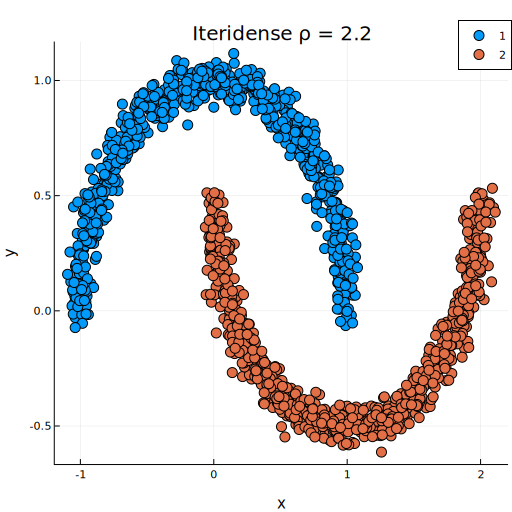
\includegraphics[scale=0.4]{clipart/Moons-Iteridense-rho2-2}
\par\end{centering}
}\hfill{}\subfloat[$\rho=5.0$, final resolution: 43]{\begin{centering}
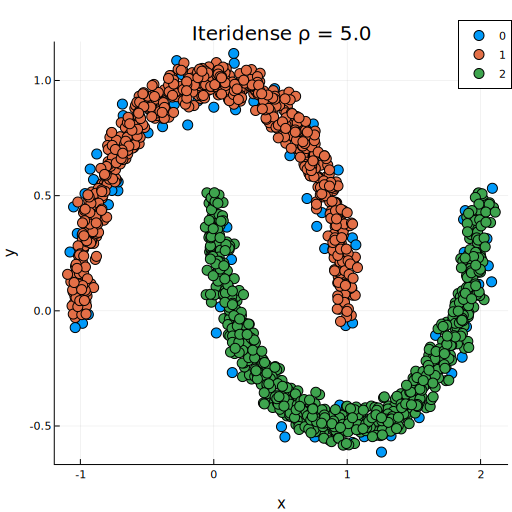
\includegraphics[scale=0.4]{clipart/Moons-Iteridense-rho5}
\par\end{centering}
}\hfill{}
\par\end{centering}
\caption{\label{fig:Result-of-the}Result of \noun{Iteridense} for intersected
moon-like clusters using different $\rho$.}
\end{figure}

By increasing $\rho$ one can for example define points as outliers:
One could define that all data points that are not part of a cluster
at density $\rho=4.0$ are outliers. If the data points are the result
of a measurement, one can repeat the measurement of an outlier point
to verify if the result is still an outlier, check the measurement
setup etc.

\ref{fig:Effect-of-a} shows the result for $\rho=6.0$. The density
is now so high that the moon-like clusters break down into many small
clusters if the option \textbf{NoDiagonals} is used for the clustering.

\begin{figure}
\begin{centering}
\hfill{}\subfloat[$\rho=6.0$, \textbf{MinClusterSize}\,=\,10 with option \textbf{NoDiagonals},
final resolution: 60]{\begin{centering}
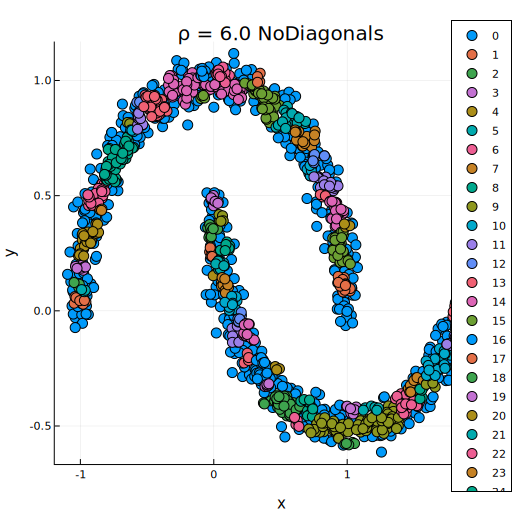
\includegraphics[scale=0.4]{clipart/Moons-Iteridense-rho6-noDiagonals}
\par\end{centering}
}\hfill{}\subfloat[$\rho=6.0$, final resolution: 52]{\begin{centering}
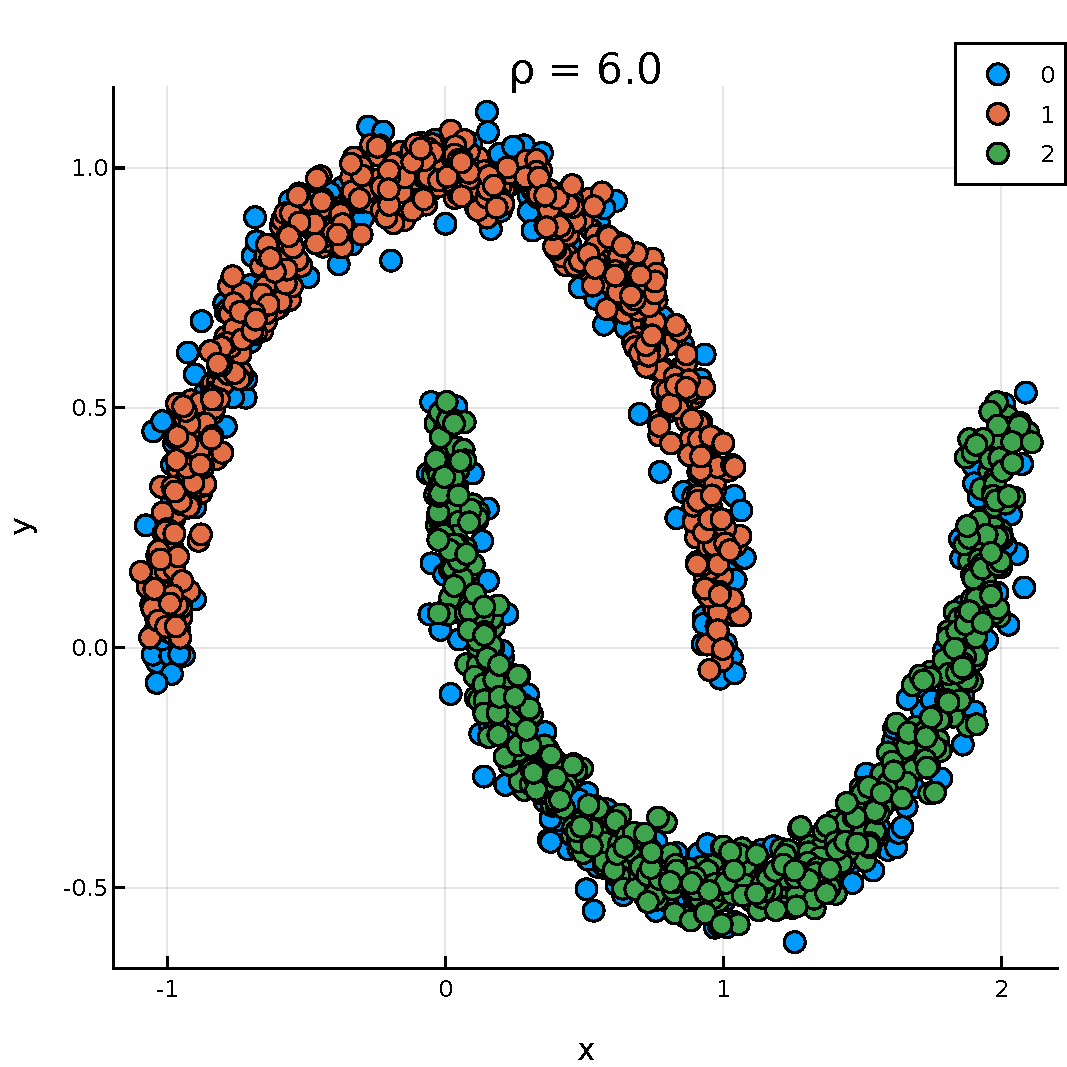
\includegraphics[scale=0.4]{clipart/Moons-Iteridense-rho6}
\par\end{centering}
}\hfill{}
\par\end{centering}
\caption{\label{fig:Effect-of-a}Effect of a high $\rho$ and the option to
evaluate neighbor cells.}
\end{figure}


\subsection{Clustering Performance\label{subsec:Clustering-Performance}}

An advantage compared to other clustering algorithm is that \noun{Iteridense}
treats all data points the same way. There is no separation between
core points, border points or the like. Another major feature of \noun{Iteridense}
is that it provides two ways to achieve results and a clear path for
the user on how to change the input parameters to get a suitable result:
\begin{itemize}
\item Either start with a low $\rho$ and increase it gradually to get a
suitable result. If the result is not suitable, look at the resulting
$\rho_{\mathrm{cluster}}$ and set for the next run $\rho$ above
their minimum.
\item Or specify with \textbf{MinClusters} the desired number of clusters.
If the result is not suitable, increase gradually either \textbf{MinClusterSize}
or \textbf{MinClusterDensity}.
\end{itemize}
The second path is computationally the fastest, as discussed in the
next section. However, it can only be taken if there is a physical
or technical reason for the number of clusters. For the path to specify
$\rho$ \ref{fig:Result-Iteridense-Blobs}\,(a)\,--\,\ref{fig:Result-Iteridense-Blobs2}\,(a)
shows the results (with \textbf{MinClusterSize}\,=\,6): Until $\rho\le6.8$
only one cluster is detected and starting at $\rho=7.3$ there are
3~clusters. Increasing $\rho$ leads to more and more clusters. This
can be used to identify regions with higher density inside a ``base''
cluster. In the example there are 3~base clusters and every one has
more dense regions that are unveiled with greater $\rho$.

\begin{figure}[p]
\begin{centering}
\hfill{}\subfloat[$\rho=6.8$, final resolution: 30]{\begin{centering}
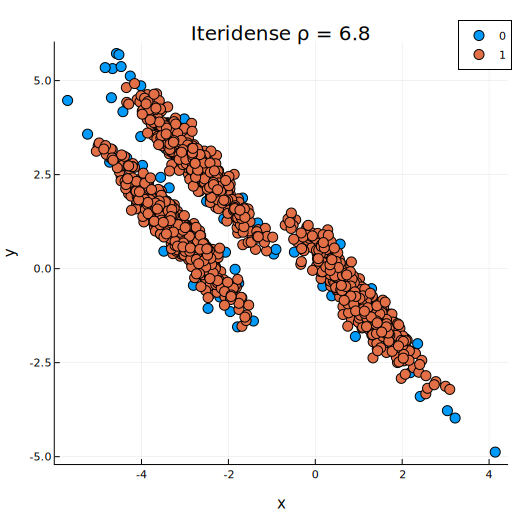
\includegraphics[scale=0.4]{clipart/Anisotropes-Iteridense-rho6-8}
\par\end{centering}
}\hfill{}\subfloat[$\rho=7.3$, final resolution: 35]{\begin{centering}
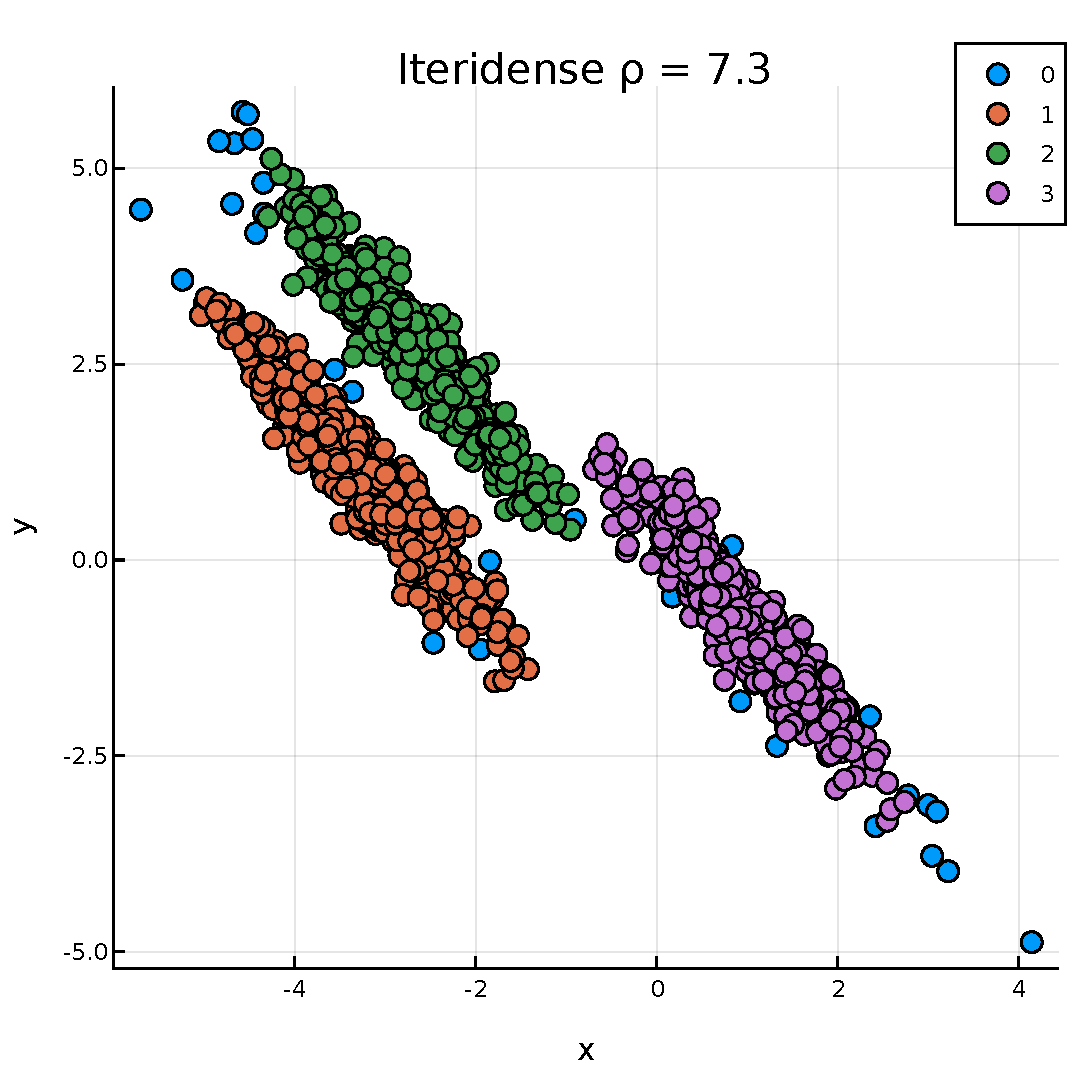
\includegraphics[scale=0.4]{clipart/Anisotropes-Iteridense-rho7-3}
\par\end{centering}
}\hfill{}
\par\end{centering}
\caption{\label{fig:Result-Iteridense-Blobs}Result of \noun{Iteridense} for
$\rho\ge6.8$ at anisotropic clusters.}
\end{figure}

\begin{figure}[p]
\begin{centering}
\hfill{}\subfloat[$\rho=12.0$, final resolution: 68]{\begin{centering}
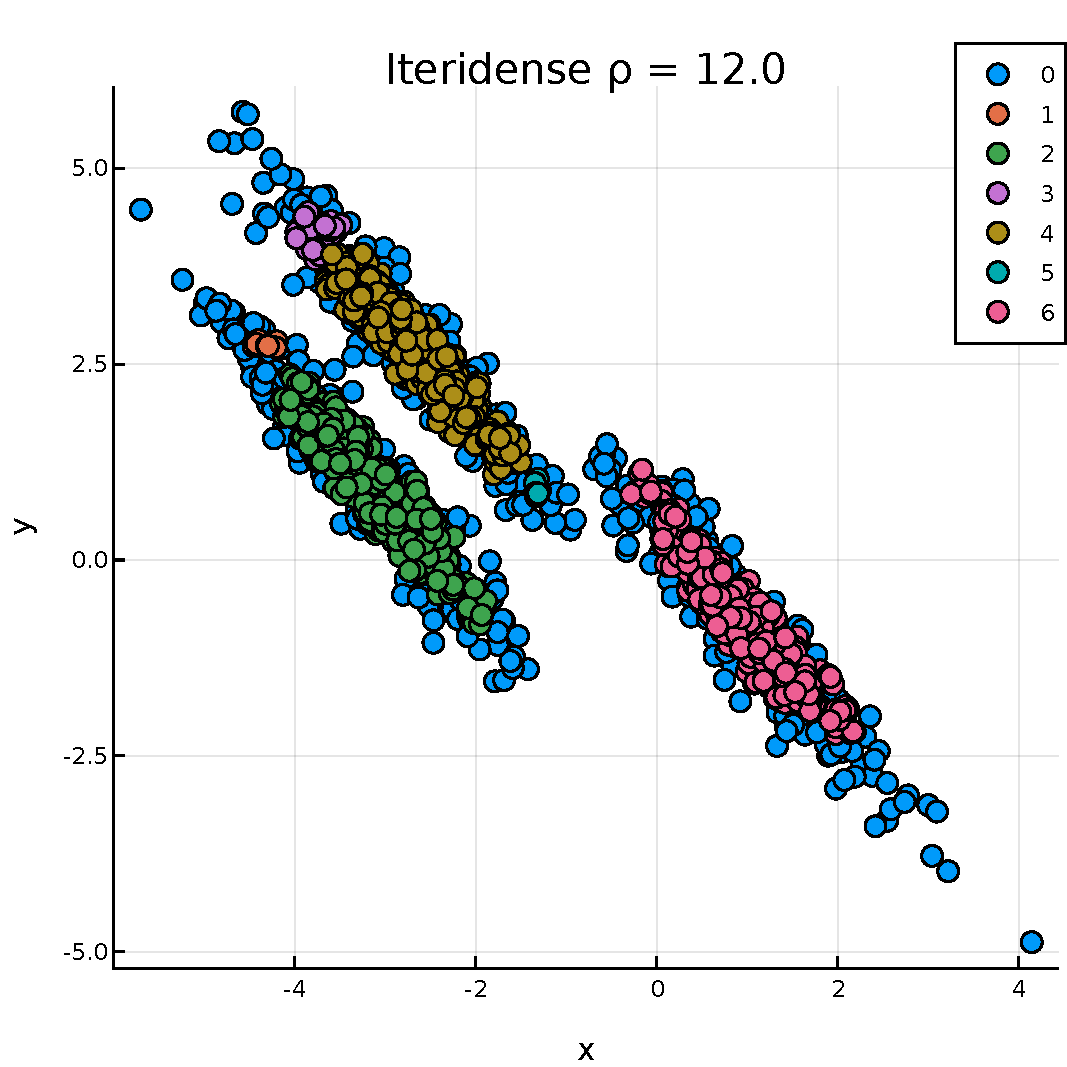
\includegraphics[scale=0.4]{clipart/Anisotropes-Iteridense-rho12}
\par\end{centering}
}\hfill{}\subfloat[$\epsilon=0.1$]{\begin{centering}
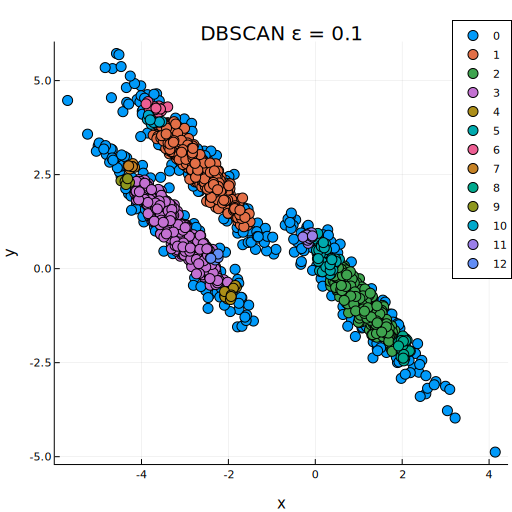
\includegraphics[scale=0.4]{clipart/Anisotropes-DBSCAN-eps0-10}
\par\end{centering}
}\hfill{}
\par\end{centering}
\caption{\label{fig:Result-Iteridense-Blobs2}Result of \noun{Iteridense} for
$\rho=12.0$ and DBSCAN for $\epsilon=0.1$ at anisotropic clusters.}
\end{figure}

For comparison, the algorithm DBSCAN does not provide a clear path
on how to change its input parameters. An example is the data shown
in \ref{fig:Result-Iteridense-Blobs2}\,(b). This data was generated
using the \emph{make\_blobs }call to \emph{sklearn.datasets} with
a subsequent transformation. Like in the previous example, there are
1500~data points. $\epsilon=0.1$ (the maximum distance to another
core point of a cluster) seems to be a sensible start value for DBSCAN.
The result is \ref{fig:Result-of-DBSCAN}\,(b). As the result is
not a useful one might increase $\epsilon$ in small steps and gets
with \textbf{MinPts} (minimal points to form a dense region) of 6
as results \ref{fig:Result-of-DBSCAN}\,--\,\ref{fig:Result-of-DBSCAN-1}.
For this dataset a human would expect 3~base clusters but DBSCAN
does not find exactly 3~clusters. One has to try different $\epsilon$
to get this result. For data in 2 or 3~dimensions one can plot the
data to get a feeling for $\epsilon$ and for example increase \textbf{MinPts}.
However, for data in higher dimensions this is hardly possible.

\begin{figure}[p]
\begin{centering}
\hfill{}\subfloat[$\epsilon=0.15$]{\begin{centering}
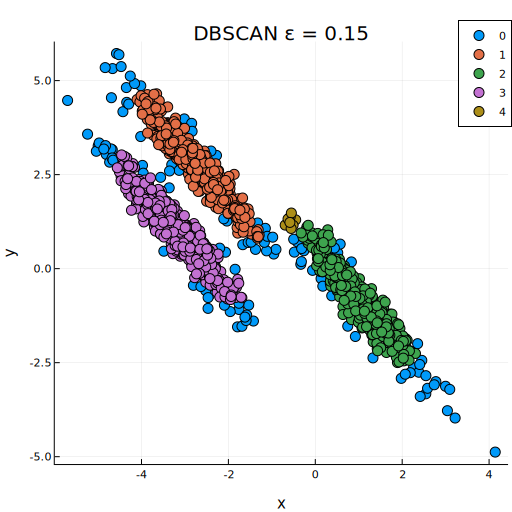
\includegraphics[scale=0.4]{clipart/Anisotropes-DBSCAN-eps0-15}
\par\end{centering}
}\hfill{}\subfloat[$\epsilon=0.2$]{\begin{centering}
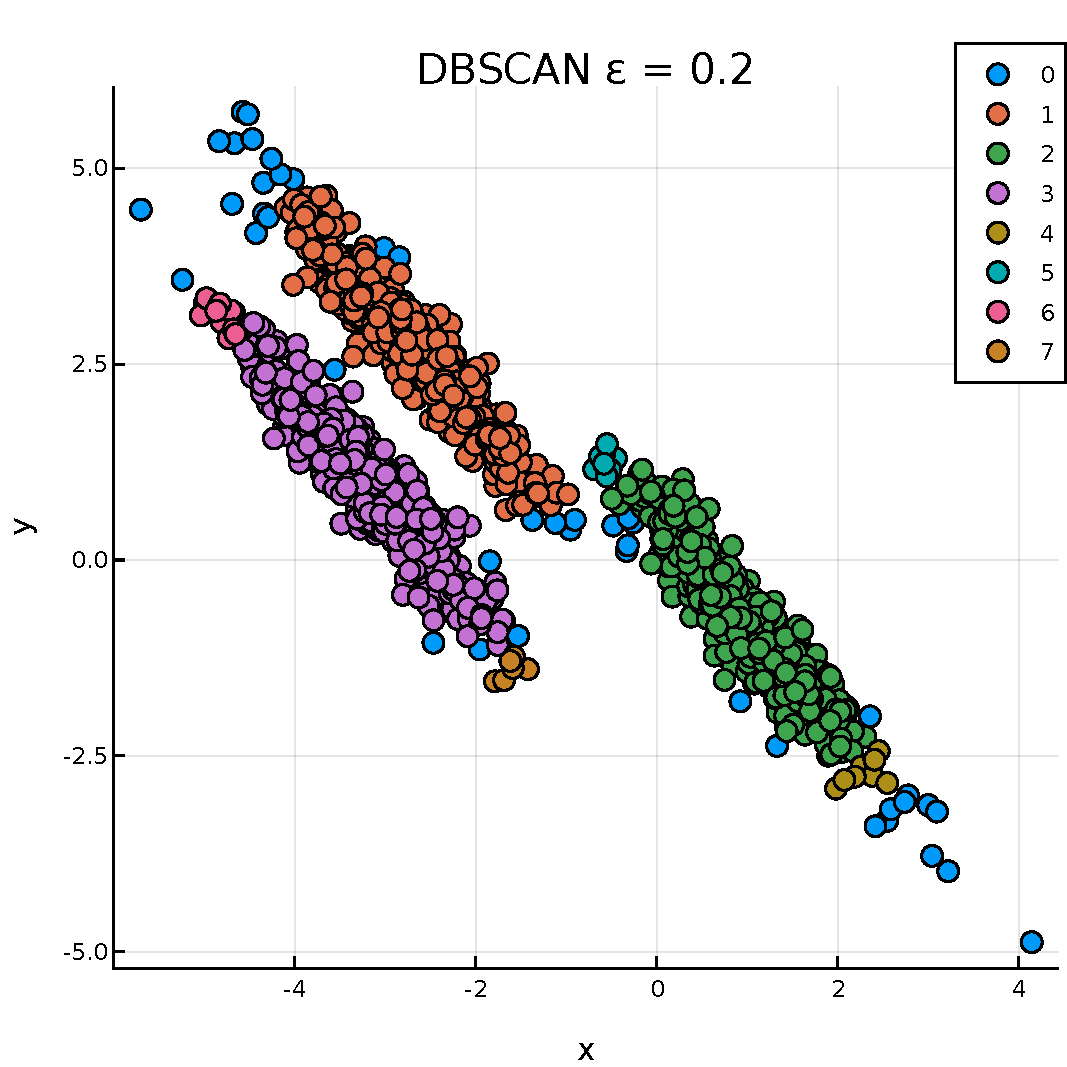
\includegraphics[scale=0.4]{clipart/Anisotropes-DBSCAN-eps0-20}
\par\end{centering}
}\hfill{}
\par\end{centering}
\caption{\label{fig:Result-of-DBSCAN}Result of DBSCAN at anisotropic clusters
with $\epsilon\le0.2$.}
\end{figure}

\begin{figure}[p]
\begin{centering}
\hfill{}\subfloat[$\epsilon=0.25$]{\begin{centering}
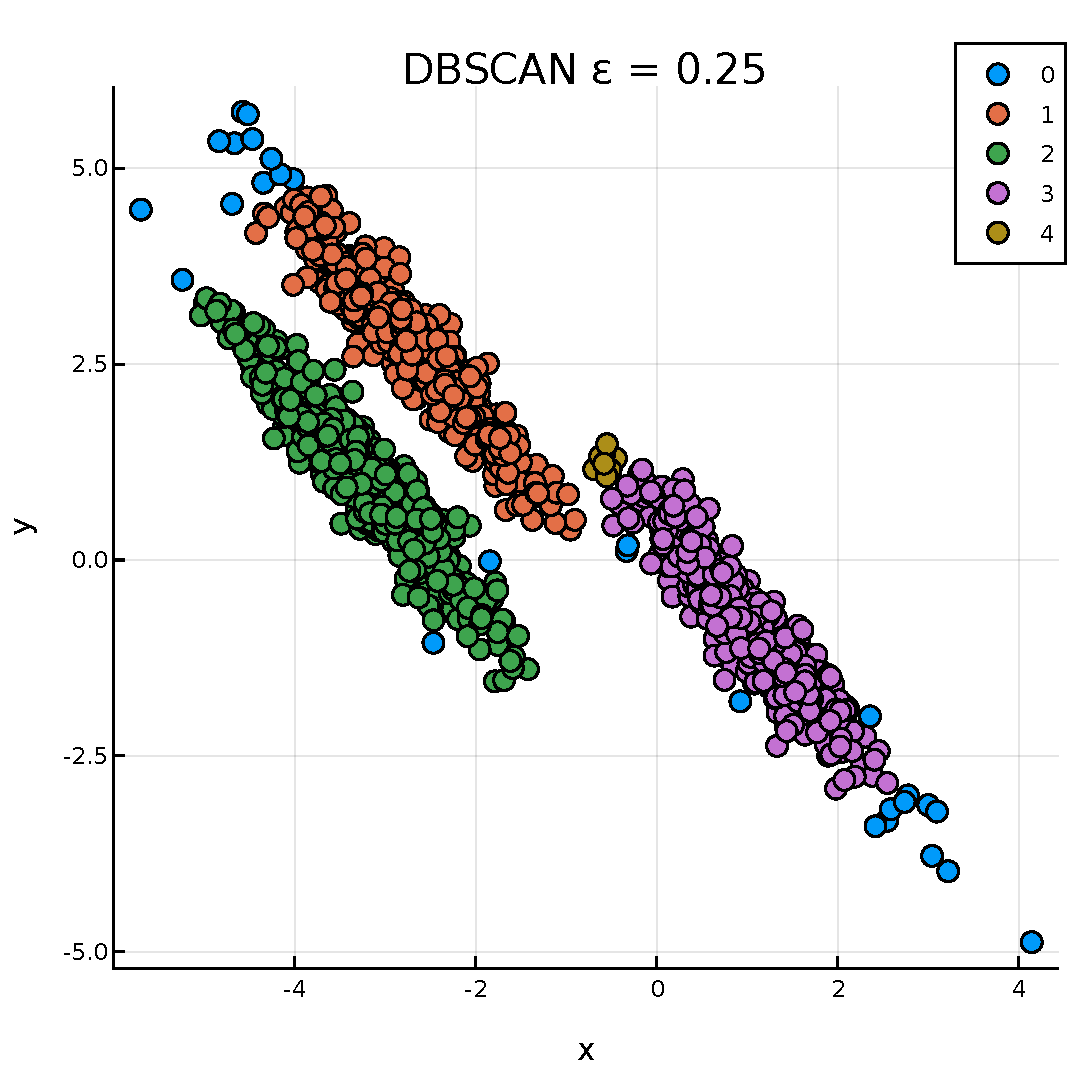
\includegraphics[scale=0.4]{clipart/Anisotropes-DBSCAN-eps0-25}
\par\end{centering}
}\hfill{}\subfloat[$\epsilon=0.3$]{\begin{centering}
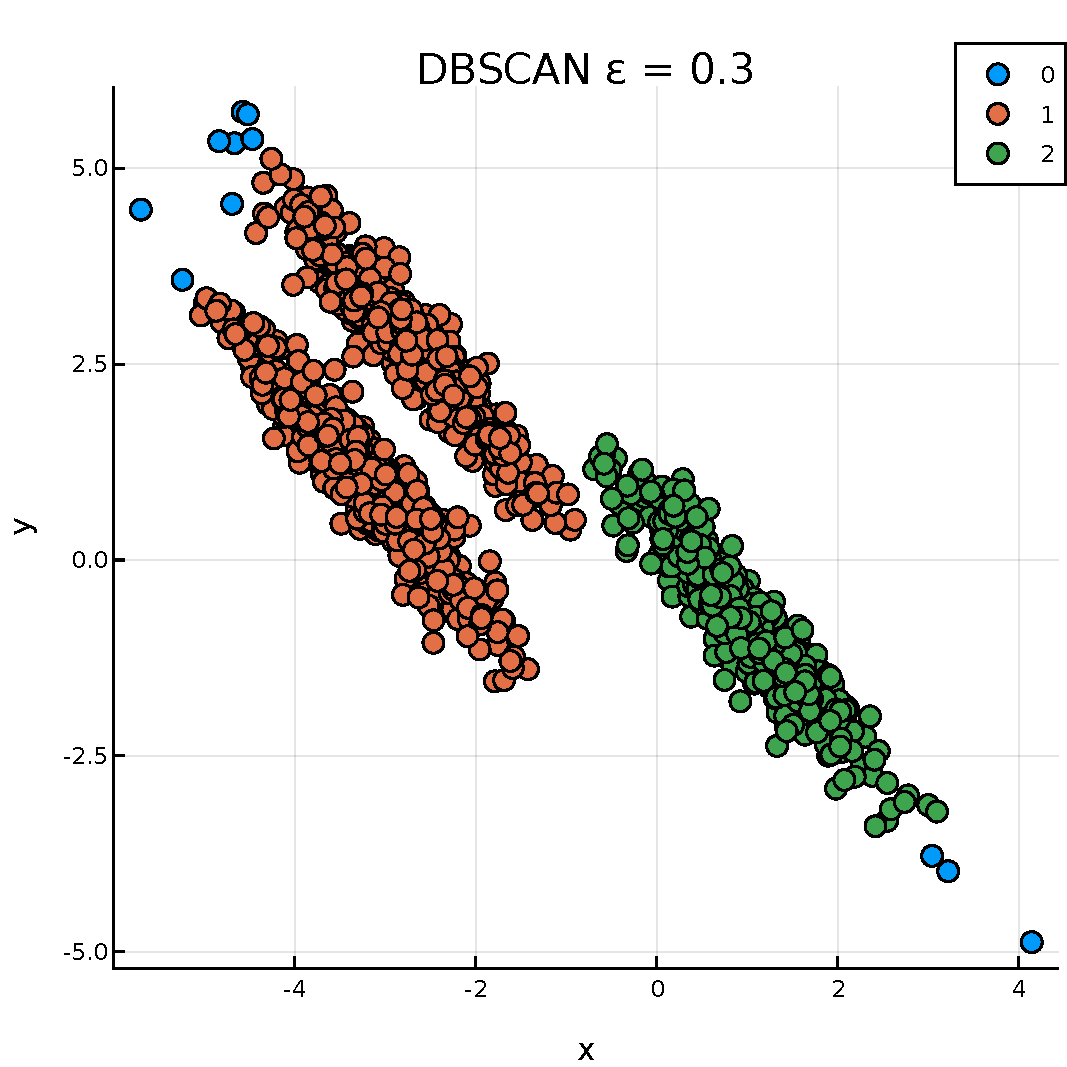
\includegraphics[scale=0.4]{clipart/Anisotropes-DBSCAN-eps0-30}
\par\end{centering}
}\hfill{}
\par\end{centering}
\caption{\label{fig:Result-of-DBSCAN-1}Result of DBSCAN at anisotropic clusters
with $\epsilon>0.2$.}
\end{figure}

What is ``suitable'' depends on the application. For example the
data shown in \ref{fig:Result-of-Iteridense-NoisyBlobs} consist also
of 1500~data points. It was generated using the \emph{make\_blobs
}call to \emph{sklearn.datasets} with a subsequent transformation.
One might see in the data 2~clusters and therefore set \textbf{MinClusters}
to 2 and \textbf{MinClusterSize} to 20. As result one gets \ref{fig:Result-of-Iteridense-NoisyBlobs}\,(a).
There cluster~1 has $\rho_{\mathrm{cluster}}=2.6$ and is a merge
of a high- and a low-density region. This might not be suitable because
one had the 2 dense regions in mind to form each a cluster. There
are now two ways to change the result:
\begin{itemize}
\item Either set \textbf{MinClusters} to 3 to get two clusters with a high
density and one with a lower density, see \ref{fig:Result-of-Iteridense-NoisyBlobs}\,(b).
\item Or increase $\rho$ and also increase \textbf{MinClusterSize} e.g.~to
50 unless one gets only 2~high-density clusters, see \ref{fig:Result-of-Iteridense-NoisyBlobs}\,(c).
Increasing \textbf{MinClusterSize} is hereby necessary to avoid small
clusters in the low-density area.
\end{itemize}
The change of \textbf{MinClusterSize} might not be obvious when one
cannot plot for example high-dimensional data. It is therefore a useful
feature of the \noun{Iteridense} algorithm that for the case $\rho_{\mathrm{cluster}}$
is too low for a suitable result, one can increase \textbf{MinClusterSize}
together with $\rho$.

\begin{figure}
\begin{centering}
\subfloat[\textbf{MinClusters} = 2]{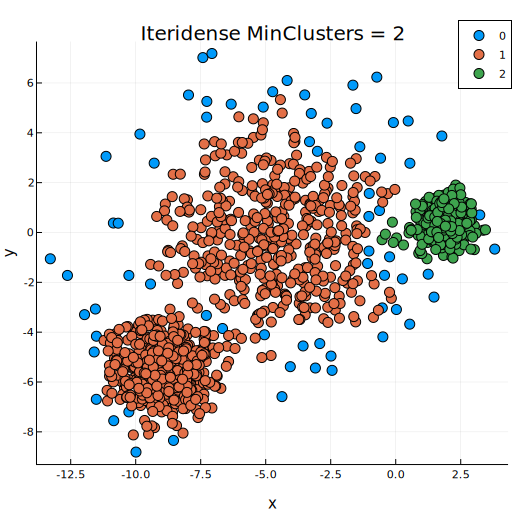
\includegraphics[width=0.33\columnwidth]{clipart/BlobNoise-Iteridense-MinClusters2}

}\subfloat[\textbf{MinClusters} = 3]{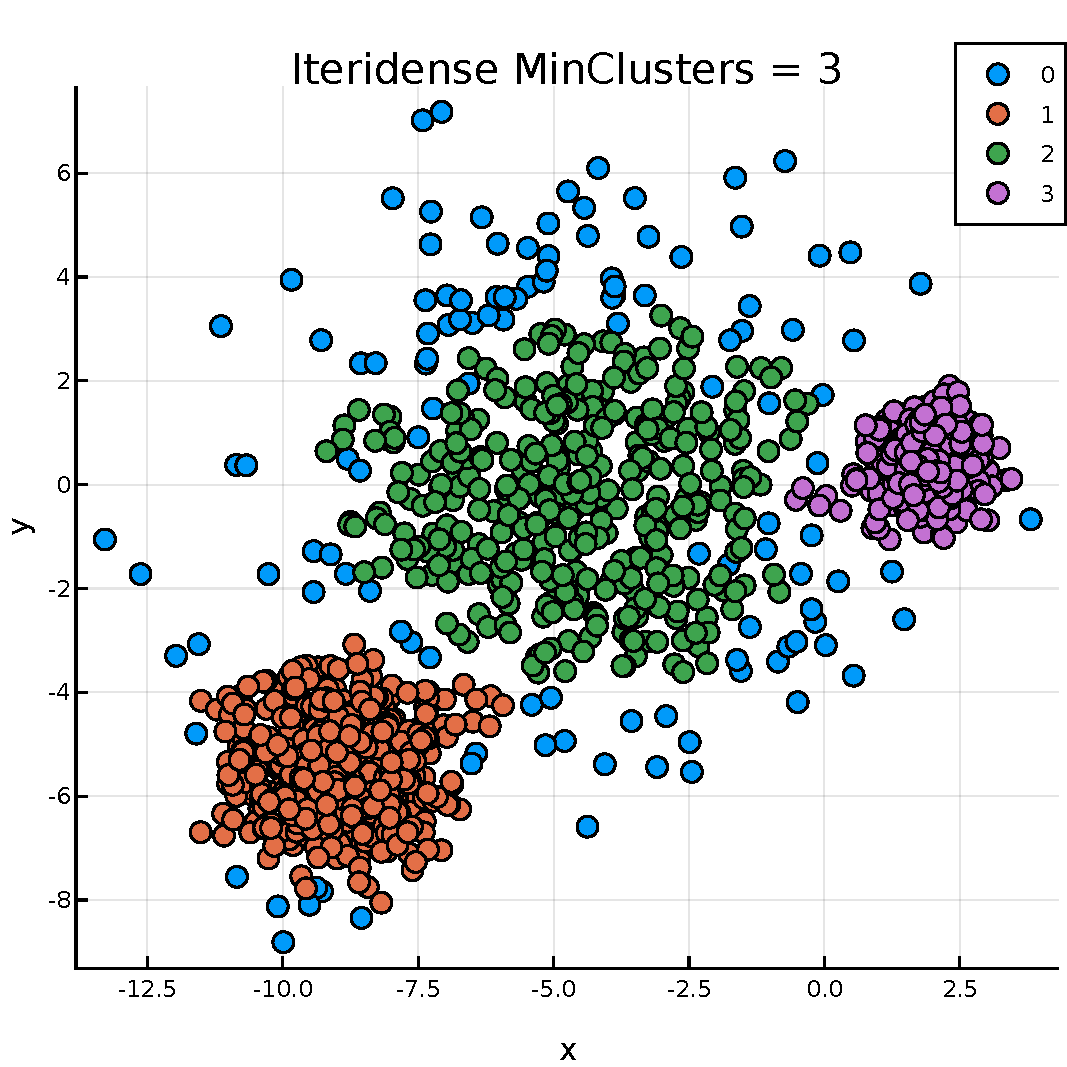
\includegraphics[width=0.33\columnwidth]{clipart/BlobNoise-Iteridense-MinClusters3}

}\subfloat[$\rho=4.0$,\protect \\
\textbf{MinClusterSize} = 50]{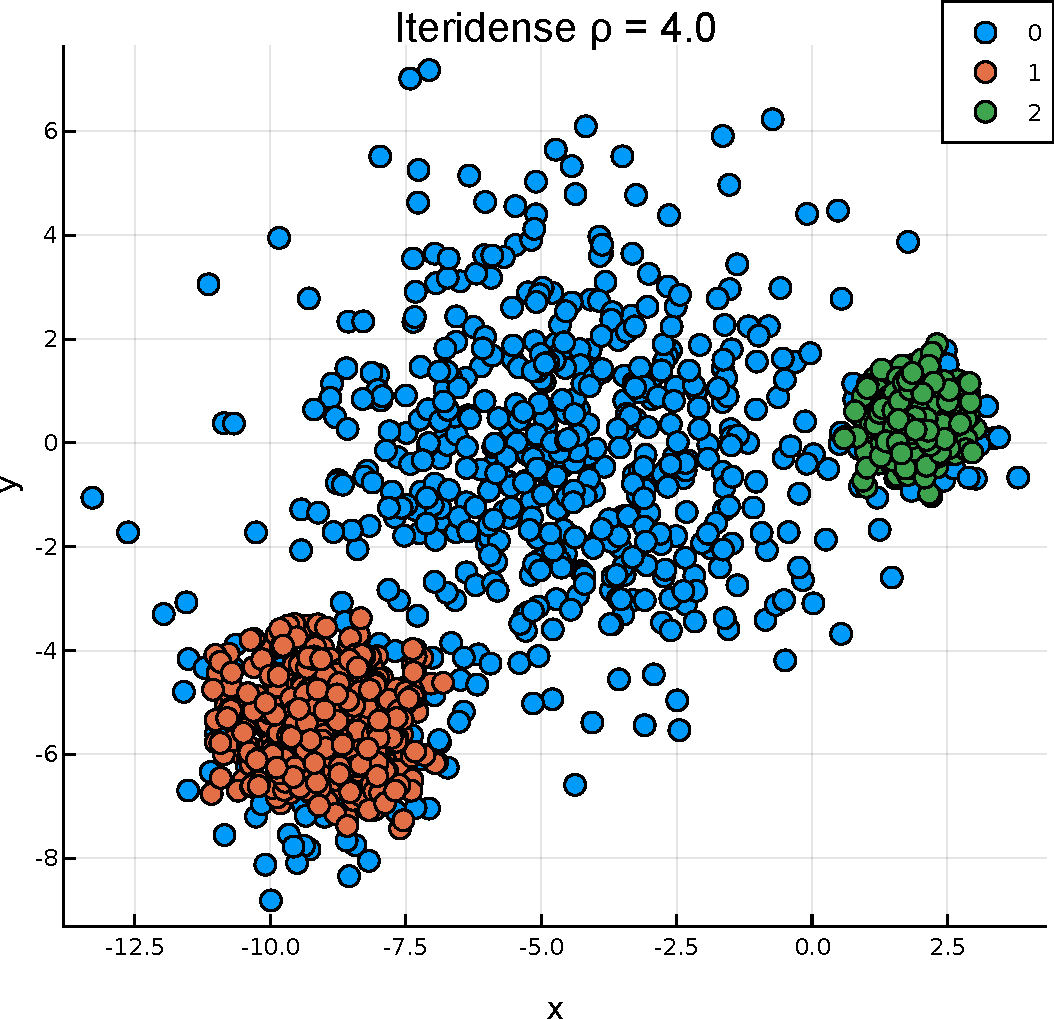
\includegraphics[width=0.33\columnwidth]{clipart/BlobNoise-Iteridense-rho4-0}

}
\par\end{centering}
\caption{\label{fig:Result-of-Iteridense-NoisyBlobs}Result of \noun{Iteridense}
for clusters with different densities.}
\end{figure}

Data with higher dimensions are a main use case for clustering algorithms
as no human could do the clustering according to plots. \ref{fig:Iteridense-Pluton}
is an example and also demonstrate the clustering performance of \noun{Iteridense}.
The data are the publicly available \emph{pluton} dataset\cite{RDataPluton}
containing concentrations of the different Plutonium isotopes in 45~ore
samples. It has 4~dimensions.

\begin{figure}
\begin{centering}
\subfloat[Clustering with only the shown\protect \\
dimensions taken into account. final resolution: 6]{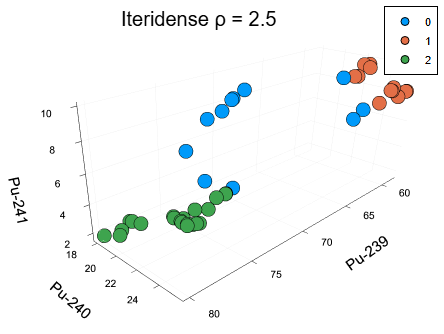
\includegraphics[width=0.33\columnwidth]{clipart/Pluto-Iteridense-rho2-5-only3}

}\subfloat[Clustering with all dimensions taken into account. final resolution:
5]{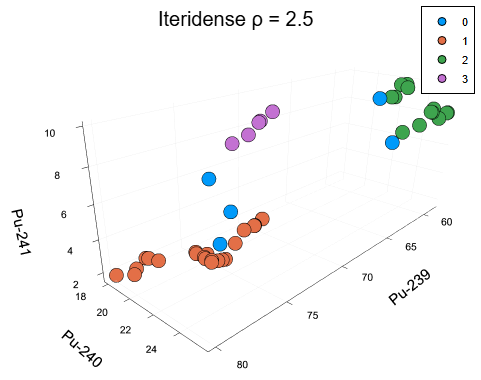
\includegraphics[width=0.33\columnwidth]{clipart/Pluto-Iteridense-rho2-5-all}

}\subfloat[like (b) but $\rho=5.9$, final resolution: 7]{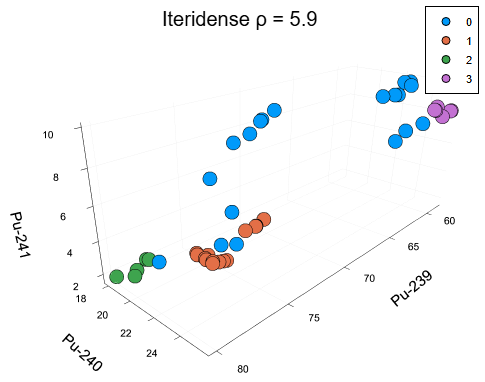
\includegraphics[width=0.33\columnwidth]{clipart/Pluto-Iteridense-rho5-9-all}

}
\par\end{centering}
\caption{\label{fig:Iteridense-Pluton}Result of \noun{Iteridense} for the
\emph{pluton} dataset.}
\end{figure}

By plotting 3~dimensions of the dataset and performing \noun{Iteridense}
only on the plotted dimensions, the result would be \ref{fig:Iteridense-Pluton}\,(a).
Taking all dimensions into account, the result is \ref{fig:Iteridense-Pluton}\,(b).
The points of high Pu-241 concentrations are then identified as a
cluster. Cluster~1 is so large because its density in all 4~dimensions
matters. If one wants for some reason cluster~1 to be split into
2~clusters, one follows the \noun{Iteridense} path and increases
$\rho$ above the lowest $\rho_{\mathrm{cluster}}$ and ends up with
\ref{fig:Iteridense-Pluton}\,(c).

\pagebreak{}

\section{Computational and Memory Complexity\label{subsec:Computational-Complexity}}

\subsection{Computational Complexity}

\noun{Iteridense} creates two tensors, the count tensor to store how
many data points are in a cell and the cluster tensor that stores
to what cluster a cell belongs to. Both tensors have the rank $D$
whereas $D$ are the dimensions of the data (or features). Each tensor
has $R^{D}$ entries (cells) whereas $R$ denote the resolution. Therefore
\noun{Iteridense} is memory-limited. This is an important point as
this limits the practical usability.

To estimate the computational complexity $\mathcal{O}$ we look at
the different steps:
\begin{lyxlist}{00.00.0000}
\item [{Counting}] Because a computation is performed for every data point
in every dimension we have $\mathcal{O}\left(DN\right)$.
\item [{Clustering}] Every cell has $B$ neighbor cells: $B=3^{D}-1$ (for
the case that option \textbf{NoDiagonals} is used $B=2D$). For the
clustering we only evaluate $B/2$ of the neighbors. Therefore checking
a neighbors has $\mathcal{O}\left(0.5BR^{D}\right)\approx\mathcal{O}\left(0.5\left(3R\right)^{D}\right)$.
\item [{Evaluation}] To evaluate how many clusters were found and how many
cells they have, all tensor cells are evaluated, therefore this step
has $\mathcal{O}\left(R^{D}\right)$.
\item [{Assignment}] To assign the cluster number to every data point the
complexity is $\mathcal{O}\left(DN\right)$.
\end{lyxlist}
\noun{Iteridense} clusters iteratively with increasing $R=R_{\mathrm{start}}\ldots R_{\mathrm{final}}+1$.
Note that the assignment is only performed once for the final $R$.
In total these are the number of computes:
\begin{align}
 & DN+\sum_{R=R_{\mathrm{start}}}^{R_{\mathrm{final}}+1}\left(DN+R^{D}\left(\frac{3^{D}}{2}+1\right)\right)\label{eq:O-initial}\\
 & \approx DN+\left(R_{\mathrm{final}}+1-R_{\mathrm{start}}+1\right)DN+\frac{3^{D}}{2}\sum_{R=R_{\mathrm{start}}}^{R_{\mathrm{final}}+1}R^{D}
\end{align}

The sum can be approximated by the integral $\int R^{D}\thinspace\mathrm{d}R$
and we can write
\begin{equation}
\sum_{R=R_{\mathrm{start}}}^{R_{\mathrm{final}}+1}R^{D}\approx\frac{\left(R_{\mathrm{final}}+1\right)^{D+1}-R_{\mathrm{start}}^{D+1}}{D+1}\label{eq:R^D-approx}
\end{equation}
For $\mathcal{O}$ we get
\begin{equation}
\mathcal{O}\left(\left(R_{\mathrm{final}}-R_{\mathrm{start}}+3\right)DN+\frac{3^{D}}{2(D+1)}\left(\left(R_{\mathrm{final}}+1\right)^{D+1}-R_{\mathrm{start}}^{D+1}\right)\right)\label{eq:O()}
\end{equation}

The worst case is $R_{\mathrm{start}}=2$ as this is the lowest possible
resolution. This leads to
\begin{equation}
\mathcal{O}_{\mathrm{worst\,case}}\approx\mathcal{O}\left(R_{\mathrm{final}}DN+\frac{3^{D}}{2(D+1)}\left(R_{\mathrm{final}}+1\right)^{D+1}\right)\label{eq:O(worst)}
\end{equation}

With this result the following can be seen:
\begin{itemize}
\item \noun{Iteridense} scales roughly with $\mathcal{O}\left(RDN+(R+1)^{D+1}\right)$
-- a linear increase plus an offset. This extends the parameter range
at which clustering could be performed, dramatically, compared to
algorithms with $\mathcal{O}\left(DN^{2}\right)$.
\item Setting $R_{\mathrm{start}}$ (the parameter \textbf{StartResolution})
has an impact, but a minor one.
\item The worst case for \noun{Iteridense} is that $\rho$ is set so high
that $R_{\mathrm{final}}=N$. To prevent that this happens, the parameter
\textbf{StopResolution} sets the limit for $R_{\mathrm{final}}$.
\end{itemize}
To prove that our derivation of $\mathcal{O}$ is correct, we took
a dataset with $N=1500$ and clustered subsets of that dataset. Every
subset has a different $N$, which allows to create a plot with the
computation time over $N$. The used dataset is shown in \ref{fig:Result-Iteridense-Circles}.
It was generated using the \emph{make\_circles }call to \emph{sklearn.datasets}.

\begin{figure}
\begin{centering}
\hfill{}\subfloat[\textbf{MinClusters} = 2, final resolution: 16]{\begin{centering}
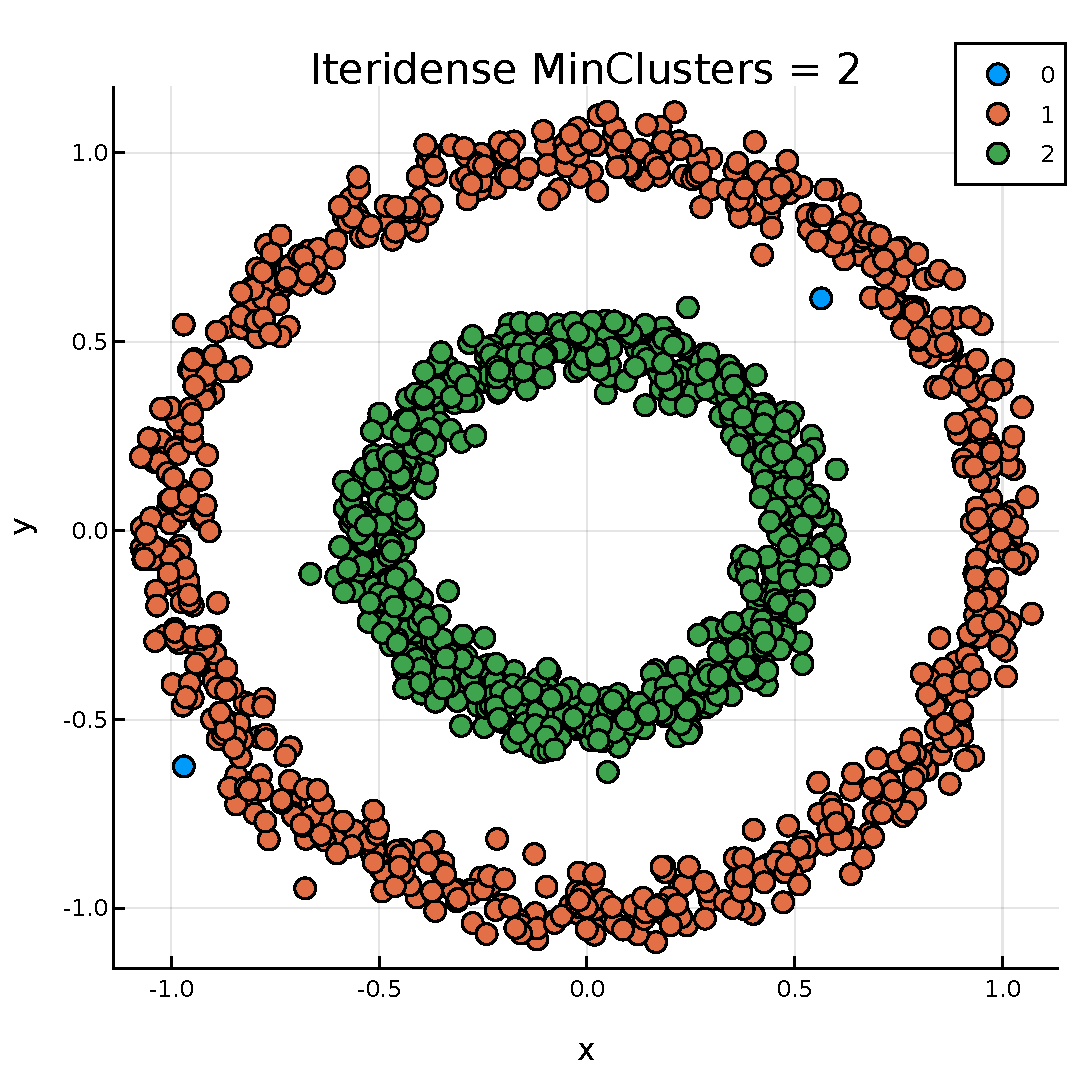
\includegraphics[scale=0.4]{clipart/Circles-Iteridense-MinClusters2}
\par\end{centering}
}\hfill{}\subfloat[$\epsilon=0.1$]{\begin{centering}
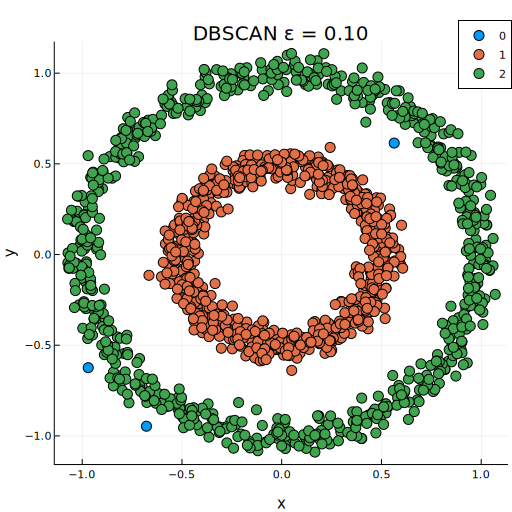
\includegraphics[scale=0.4]{clipart/Circles-DBSCAN-eps0-1}
\par\end{centering}
}\hfill{}
\par\end{centering}
\caption{\label{fig:Result-Iteridense-Circles}Result of \noun{Iteridense}
and DBSCAN for intersected circle-like clusters.}
\end{figure}

\ref{fig:Result-Iteridense-Circles}\,(a) shows the \noun{Iteridense}
result for the full dataset for $\text{\textbf{MinClusters}}=2$.
Thereby $R_{\mathrm{final}}=16$ and this value was used for \textbf{StopResolution}
when clustering the subsets. By setting $\text{\textbf{MinClusters}}=20$
it was assured that for every clustering $R_{\mathrm{final}}=16$
was reached.\\
For comparison, \ref{fig:Result-Iteridense-Circles}\,(b) shows the
result using the DBSCAN algorithm for $\epsilon=0.1$ and $\text{\textbf{MinPts}}=3$.
We chose for the subset clustering also $\epsilon=0.2$ to see the
influence of $\epsilon$ on the computation time.\\
The computation of the k-mean and DBSCAN algorithms were performed
using their implementation in the package \emph{Clustering} of the
\noun{Julia} programming language, \cite{ClusteringDBSCAN}. The times
were measured using the feature \emph{@elapsed} of the \noun{Julia}
programming language. To get reliable values, the clustering was for
every algorithm performed 2000~times in a row and the overall time
was taken.

The result is shown in \ref{fig:Computation-time-comparison}\,(a).
\noun{Iteridense} shows the same linear increase as k-means proving
that formula \eqref{eq:O(worst)} is basically correct. The slope
of the increase is relatively low. For DBSCAN in the used implementation,
one can see that is has $\mathcal{O}\left(DN^{2}\right)$ and how
the choice of $\epsilon$ influences the computation time.

\begin{figure}
\begin{centering}
\subfloat[$D=2$]{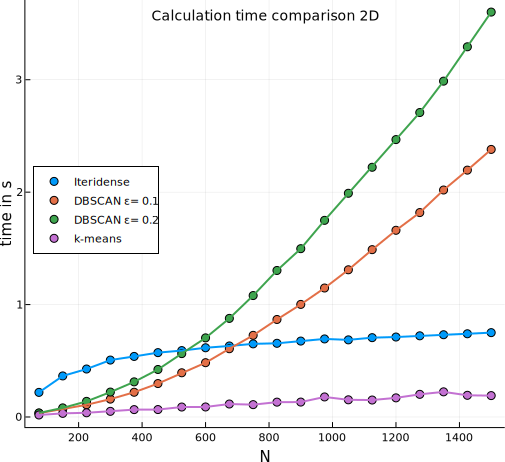
\includegraphics[width=0.49\columnwidth]{clipart/Calculation-time-comparison-2D}

}\subfloat[$D=3$]{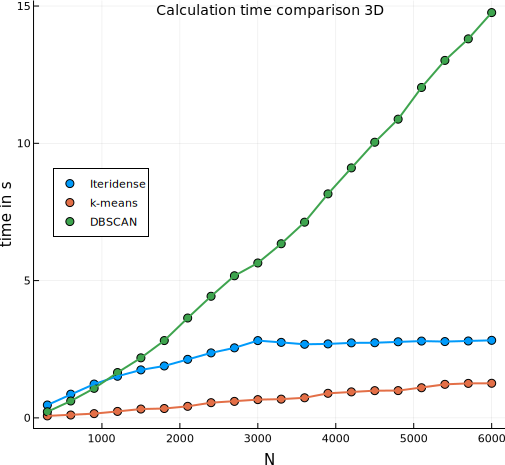
\includegraphics[width=0.49\columnwidth]{clipart/Calculation-time-comparison-3D}

}
\par\end{centering}
\caption{\label{fig:Computation-time-comparison}Computation time comparisons
for 2 similar datasets. The computations were performed using the
CPU \noun{AMD Ryzen 9 9900X}.}
\end{figure}

The $N$ at which \noun{Iteridense} is faster than DBSCAN is at about
$N=470$. By repeating the test in 3D, there should be an increase
of this value because of the greater offset in $\mathcal{O}$ for
\noun{Iteridense}. This test was performed by adding z-values to the
dataset so that the clusters form cylinders. DBSCAN finds the 2~clusters
for the range $0.2\le\epsilon\le0.26$ and we chose the lowest possible
$\epsilon=0.2$. Eventually, we extended the dataset by multiplying
its points to get in total $N=6000\thinspace$points. The result is
shown in \ref{fig:Computation-time-comparison}\,(b). The $N$ at
which \noun{Iteridense} is faster than DBSCAN is now at about $N=1100$.

\begin{figure}
\begin{centering}
\hfill{}\subfloat[\textbf{MinClusters} = 2, final resolution: 13]{\begin{centering}
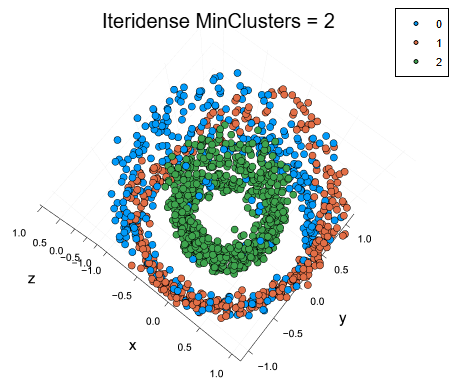
\includegraphics[width=0.45\columnwidth]{clipart/Circles3D-Iteridense}
\par\end{centering}
}\hfill{}\subfloat[$\epsilon=0.2$]{\begin{centering}
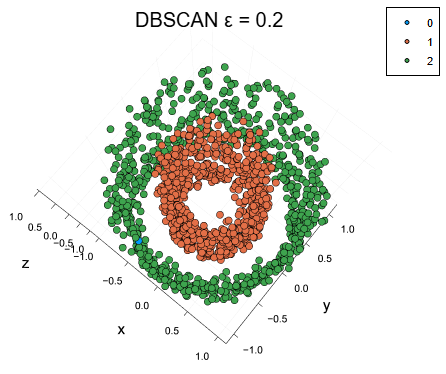
\includegraphics[width=0.45\columnwidth]{clipart/Circles3D-DBSCAN-eps0-2}
\par\end{centering}
}\hfill{}
\par\end{centering}
\caption{\label{fig:Result-Iteridense-Cylinders}Result of \noun{Iteridense}
and DBSCAN for intersected cylinder-like clusters.}
\end{figure}

\ref{fig:Result-Iteridense-Cylinders} shows the cluster result for
the full 3D dataset for $\text{\textbf{MinClusters}}=2$. \noun{Iteridense}
does not find the outer cylinder to be completely a cluster. DBSCAN
can find it because it allows to change the search radius. However,
it took several cluster attempts to find an $\epsilon$ that works.
In 3D the dataset can be visualized to find a suitable $\epsilon$
but this is impossible in higher dimensions. In effect DBSCAN provides
for this task more flexibility and a more suitable result for the
cost that one needs to try. In comparison, for \noun{Iteridense} one
can set $\text{\textbf{MinClusters}}=2$ and then fine-tune with $\rho$.
This dataset is a good example that every algorithm has its strengths
and weaknesses.

\subsection{Memory Complexity\label{subsec:Memory-Complexity}}

The main limitation of \noun{Iteridense} is its basic memory complexity
of $\mathcal{O}\left(R^{D}\right)$. Therefore on consumer hardware
the practical limit would be with $R=10$ around $D\approx11$.\footnote{Assuming \noun{Iteridense} uses the data type Float32 (size 4~byte)
for the tensors.} However, for many datasets several dimensions are categorical data.
Therefore it is not necessary to create the count tensor with $R^{D}$
cells. For example if one dimension is the gender, there are only
3 cells necessary to store the information of this dimension, 2 for
the gender and 1 to separate both.

For this case the \noun{Iteridense} algorithm has the option \textbf{OmitEmptyCells}.
If used, the tensor will have 
\begin{equation}
R^{D-D_{c}}\cdot\bar{K}^{D_{c}}
\end{equation}
 cells, whereas $D_{c}$ is the number of dimensions with categorical
data and $\bar{K}$ is the mean number of categories in the categorical
dimensions of the dataset.

This option increases the applicability of Iteridense significantly.
Because a dataset with e.\,g. $D_{c}={\displaystyle \frac{D}{2}}$
and $\bar{K}=3$ can be clustered on consumer hardware for $R=10$
up to $D=14$.

The determination of the necessary number of cells per dimension has
$\mathcal{O}\left(DN\left(1+\log(N)\right)\right)$. For the clustering
step of the algorithm there are not $R^{D}$ cells, thus $\approx\mathcal{O}\left(0.5\cdot3^{D}R^{D-D_{c}}\cdot\bar{K}^{D_{c}}\right)\vphantom{\bar{K}^{D_{c}^{D^{D}}}}$.
Therefore \eqref{eq:O-initial} changes to 
\begin{align}
 & DN+\sum_{R=R_{\mathrm{start}}}^{R_{\mathrm{final}}+1}\left(DN\log(N)+DN+R^{D-D_{c}}\cdot\bar{K}^{D_{c}}\left(\frac{3^{D}}{2}+1\right)\right)
\end{align}

Using \eqref{eq:R^D-approx} this leads with the worst case $R_{\mathrm{start}}=2$
to
\begin{equation}
\mathcal{O}_{\mathrm{worst\,case}}\approx\mathcal{O}\left(DN+R_{\mathrm{final}}DN\left(1+\log(N)\right)+\frac{3^{D}\bar{K}^{D_{c}}}{2(D-D_{c}+1)}\left(R_{\mathrm{final}}+1\right)^{D-D_{c}+1}\right)\label{eq:O-omitEmptyCells}
\end{equation}

In effect clustering with the option \textbf{OmitEmptyCells} scales
roughly with
\begin{equation}
\mathcal{O}\left(RDN\left(1+\log(N)\right)+(R+1)^{D-D_{c}+1}\bar{K}^{D_{c}}\right)
\end{equation}
Comparing this with \eqref{eq:O()}, shows that clustering will then
have a $\left(1+\log(N)\right)$ times greater linear increase of
the computation time with increasing number of data points. This can
be seen in \ref{fig:Computational-time-6D} that shows the computation
time of a dataset with $D=6$, $D_{c}=3$ and $\bar{K}=2.66$.

\begin{figure}
\begin{centering}
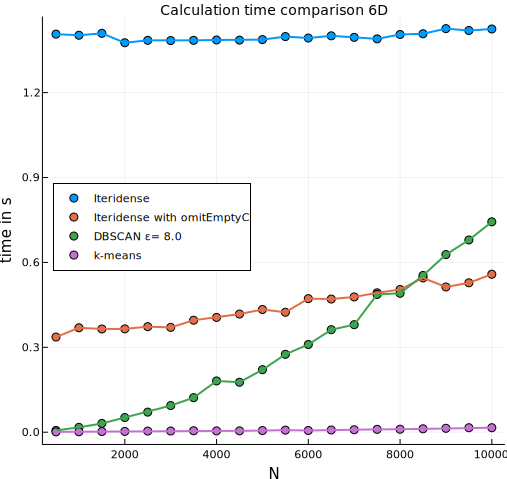
\includegraphics[width=0.49\columnwidth]{clipart/Calculation-time-comparison-6D}
\par\end{centering}
\caption{\label{fig:Computational-time-6D}Computation time comparison for
a dataset with $D=6$, $D_{c}=3$ and $\bar{K}=2.66$.}
\end{figure}

In effect the greater memory efficiency with the option \textbf{OmitEmptyCells}
has computation costs but these are still linear. Thus \noun{Iteridense}
outperforms also in this case algorithms with $\mathcal{O}\left(DN^{2}\right)$.
For comparison \ref{tab:Computational-and-memory} lists $\mathcal{O}$
of different clustering algorithms.

\begin{table}[h]
\caption{\label{tab:Computational-and-memory}Computational and memory complexity
for different cluster algorithms.}

\centering{}%
\begin{tabular}{ccc}
\toprule 
Algorithm & Computational Complexity & note\tabularnewline
\midrule
\midrule 
\noun{Iteridense} & $\mathcal{O}\left(RDN+(R+1)^{D+1}\right)$ or $\mathcal{O}\left(RDN\left(1+\log(N)\right)+(R+1)^{D-D_{c}+1}\bar{K}^{D_{c}}\right)$ & see formulas \eqref{eq:O()}, \eqref{eq:O-omitEmptyCells}\tabularnewline
\midrule 
DBSCAN & $\mathcal{O}(DN\log N)$ to $\mathcal{O}\left(DN^{2}\right)$ \cite{Chen2025} & $\mathcal{O}\left(DN^{2}\right)$ if brute force\tabularnewline
\midrule 
DENCLUE & $\mathcal{O}(DN\log N)$ to $\mathcal{O}\left(DN^{3}\right)$ \cite{Ajmal2024} & $\mathcal{O}\left(N^{3}\right)$ worst case for $N$ iterations\tabularnewline
\midrule 
k-means & $\mathcal{O}(DN)$ \cite{Ahmed2020} & \tabularnewline
\bottomrule
\end{tabular}
\end{table}


\section{Discussion}

As shown, the \noun{Iteridense} algorithm is applicable for general
purposes. It is more computation-efficient than pure density-based
algorithms that evaluate neighboring data points. But it shares with
density-based algorithms the drawback that clusters overlapping each
other cannot be detected. For example it will perform as poor as DBSCAN
on Fisher's Iris dataset, \cite{Fisher1936}.

\noun{Iteridense} shows some similarities to the grid-based DENCLUE
algorithm. However, the assignments of the data points to the clusters
is different because\linebreak{}
 DENCLUE assumes a Gaussian distribution function as shape of the
density function. Another big difference to DENCLUE is that there
is not only a single probability-density function created but iteratively
several ones with increasing resolution. This increases the computation
efforts for the benefit that one does not need to make assumptions
about the density in the dataset. DENCLUE requires at least 2~input
variables. $\xi$ is similar to $\rho$ in \noun{Iteridense}. The
parameter $\sigma$ defines the width of the Gaussian that is used
to assign the data points to the clusters. Its value has to be guessed
and therefore introduces for some practical applications a trial and
error process. There are approaches to improve the initial setting
of the DENCLUE parameters, see~\cite{Ajmal2024}, but in general
this will remain as a practical challenge.

Compared to the grid-based algorithm CLIQUE, \noun{Iteridense} does
not require to specify the size of the cell (CLIQUE's parameter $\xi$)
since the cell width is iteratively approached. There is also no need
to specify the number of data points in a cell to treat the cell as
being part of a cell (CLIQUE's parameter $\tau$). The \noun{Iteridense
}algorithm treats every cell with at least 2~data points as part
of a cluster. This is possible because at the end of every loop (steps~\ref{enu:AlgoStep1}\,--\,\ref{enu:AlgoStep5})
the clusters are evaluated and if their $\rho_{\mathrm{cluster}}$
is too low, the cluster is deleted. This is an advantage to CLIQUE
because especially for high-dimensional data it is hard to estimate
how many data points might end up in a cell.

\noun{Iteridense} is a simple algorithm: The user does not need to
estimate in advance a cell size, how many data points will be in a
cell, the mean distance between data points in a cluster or the like.
One can either specify \textbf{MinClusters} or $\rho$ , sets \textbf{MinClusterSize}
and gets in many cases directly a suitable result. If necessary, \noun{Iteridense}'s
clear path on how to change the input parameters guides the user to
more suitable or different results.

\section{Conclusions}

This paper introduced \noun{Iteridense}, an iterative clustering algorithm
combining grid-based and density-based methods. As result no point
in a dataset can be in more than one cluster. In contrary to k-Means
and Gaussian mixture clustering, points can also remain as not being
part of any cluster.

\noun{Iteridense} is simple to use because it does not require to
estimate settings in advance and because it provides two ways to run
the clustering. For both ways there is a clear path on how to change
the algorithm's input parameters to achieve suitable results. \noun{Iteridense}
provides different options to affect the clustering result.

The \noun{Iteridense} algorithm has a $\mathcal{O}\left(DN+R^{D+1}\right)$
and therefore extends the application range compared to algorithms
having $\mathcal{O}\left(DN^{2}\right)$. Compared to pure grid-based
algorithms it has the advantage that the user does not have to make
assumptions on how the grid should be defined or about the shape of
the probability-distribution.

It was demonstrated that for common example datasets \noun{Iteridense}
performs clustering as good to the DBSCAN algorithm with less computational
effort.

We provide online a reference implementation together with an example
worksheet, \cite{Iteridense}. We also provide a stand-alone program
with a graphical user interface that can be used to cluster any data
that is available as a CSV file, \cite{Iteridense-package}.

\printbibliography[heading=bibintoc]

\end{document}
